\part[author={\protect\insertauthor},label={chap:intermediate_code_generation}]{Semantic Analysis and Intermediate Code Generation}

\begin{graphicspathcontext}{{./chapters/chapter4/imgs/auto/},{./chapters/chapter1/imgs/auto/}}
	\begin{bibunit}[apalike]

\tableofcontentslide

\section{Introduction}
\sectiontableofcontentslide

\begin{rightlawnframe}<12>{{Semantic Analysis} and Intermediate Code Generation}{code-generator-introduction}
	\putat*(340,-197){\includeanimatedfigure[width=2.5cm]{compiler_structure}}
	Translation of languages guided by context-free grammars \\[.2cm]
	\emph{Type checking} for source language \\[.2cm]
	\emph{Generation} of parse tree or intermediate code \\[.2cm]
	\emph{Parse tree} is an abstract representation of the program \\[.2cm]
	\emph{Intermediate code} is assembly language independent of any platform
\end{rightlawnframe}

\sidecite{Samelson.1960, Brooker.1962, Paakki.1995}
\begin{frame}{Syntax-Directed Translation}
	\begin{itemize}
	\item \emph{Syntax-directed translation} specifies the values of attributes, attached to the grammar symbols, by associating semantic rules with the grammar productions \\[.2cm]
		\begin{sdd}
		\sddtitle{Grammar Productions}{Semantic Rules}
		\sddprod{expr}{\sddpn{expr} \; \sddts{+} \; \sddpn{term}}{head.t = expr.t \concat term.t \concat '+'}
		\sddalt{\sddpn{expr} \sddts{-} \sddpn{term}}{head.t = expr.t \concat term.t \concat '-'}
		\sddalt{\sddpn{term}}{head.t = term.t}
		\sddprod{term}{\sddts{0}}{head.t = '0'}
		\sddalt{\sddts{1}}{head.t = '1'}
		\sdddots
		\sddalt{\sddts{9}}{head.t = '9'}
		\end{sdd}
	\vspace{1em}
	\item Semantic rules are program fragments (or semantic actions, between braces)
	\end{itemize}
\end{frame}

\begin{frame}{{Two Types} of Syntax-Directed Translation}
	\begin{rightarrowsequence}
		\arrow{Construct a parse tree}
		\arrow{Compute the attributes' values of the tree nodes}
	\end{rightarrowsequence}
	\vspace{.2cm}
	\begin{center}
		\titlebox*[.3\linewidth]{L-attributed Translations}{L=left}
		\hspace{1cm}
		\titlebox*[.3\linewidth]{S-attributed Translations}{S=synthesized}
	\end{center}
	\vspace{.25cm}
	\alertbox*{In many cases, translation can be done during parsing, without building an explicit tree in memory}
\end{frame}

\begin{frame}{Program Checking}
	\begin{center}
		\fancybox{Type Checking}{Ensures that operators are applied to compatible operands}{type-checking}{}
		\hspace{1cm}
		\fancybox{Syntactic Checking}{Apply additional syntactic check that are not done by the syntax analyzer}{syntactic-checking}{}
	\end{center}
\end{frame}

\begin{frame}{Intermediate Representation}
	\alertbox*{In translating a program to target machine code, a compiler may construct a sequence of intermediate representations}
	\vspace{.25cm}
	\pgfuseimage{intermediate-representations}
	\vspace{.25cm}
	\begin{center}
		\simplebox*[.4\linewidth]{High-level representation is close to the source language, e.g., syntax tree}
		\hspace{1cm}
		\simplebox*[.4\linewidth]{Low-level representation are close to the target machine, e.g., three-address code}
	\end{center}
\end{frame}

\section{Translation scheme}
\sectiontableofcontentslide*

\subsection{Syntax-directed definition}
\subsectiontableofcontentslide

\begin{frame}{Syntax-Directed Definition}
	\begin{definitionblock}{Syntax-Directed Definition --- SDD}
		Context-free grammar together with attributes and semantic rules
	\end{definitionblock}
	\begin{description}
	\item[Attribute] is associated with grammar symbol
	\item[Semantic Rule] is associated with production
	\end{description}
	\vfill
	\begin{sdd}
	\sddtitle{Productions}{Semantic Rules}
	\sddprod{expr}{\sddpn{expr} \; \sddts{+} \; \sddpn{term}}{head.t = expr.t \concat term.t \concat '+'}
	\sddalt{\sddpn{expr} \; \sddts{-} \; \sddpn{term}}{head.t = expr.t \concat term.t \concat '-'}
	\sddalt{\sddpn{term}}{head.t = term.t}
	\sddprod{term}{\sddts{0}}{head.t = '0'}
	\sddalt{\sddts{1}}{head.t = '1'}
	\sdddots
	\sddalt{\sddts{9}}{head.t = '9'}
	\end{sdd}
\end{frame}

\begin{frame}{{Two Notations} for Syntax-Directed Definition}
	\begin{itemize}
	\item Notation during the lectures:
		\begin{sdd}
		\sddtitle{Productions}{Semantic Rules}
		\sddprod{A}{\sddpn{B} \; \sddpn{C}}{First part of Rule 1}
		\sddmore{D \; E}{Second part of Rule 1}
		\sddalt{\sddpn{F}}{Rule 2}
		\sddprod{G}{\sddpn{H} \; \sddpn{I} \; \sddpn{J}}{Rule 3}
		\end{sdd}
	\vfill
	\item Notation during the tutorial sessions and labworks:
		\begin{tabularx}{\linewidth}{|lcX|}
		\hline
		$\sddpn{A}$ & $\sddpo$ & $\sddpn{B} \; \sddpn{C}$ \texttt{\{ First part of Rule 1 \}} $\sddpn{D} \; \sddpn{E}$ \texttt{\{ Second part of Rule 1 \}} \\
		& $\sddor$ & $\sddpn{F}$ \texttt{\{ Rule 2 \}} \\
		$\bnfpn{G}$ & $\sddpo$ & $\sddpn{H} \; \sddpn{I} \; \sddpn{J}$ \texttt{\{ Rule 3 \}} \\
		\hline
		\end{tabularx}
	\end{itemize}
\end{frame}

\subsection{Attributes of the productions}
\subsectiontableofcontentslide

\begin{frame}{Attributes}
	\begin{definitionblock}{Attribute}
		Any quantity associated with a programming construct \\[.5cm]
		Since we use grammar symbols (terminals and nonterminals) to represent programming constructs, notion of attribute is extended from constructs to the symbols that represent them
	\end{definitionblock}
	\vspace{.5cm}
	\begin{examples}
		Data types, number of instructions, line of the first occurrence of an identifier\dots
	\end{examples}
\end{frame}

\begin{frame}{Notation for Attributes}
	\begin{itemize}
		\item In this lecture, attributes are written following one of the notations: \\[.25cm]
			\simplebox{\texttt{{\textless}terminal{\textgreater}.{\textless}attribute name{\textgreater}}}
			\simplebox{\texttt{{\textless}nonterminal{\textgreater}.{\textless}attribute name{\textgreater}}}
		\item Keyword ``\texttt{head}'' represents the nonterminal in the production's head
		\item If the same nonterminal is present many times in the body, the attribute's prefix is indexed by the position of the nonterminal in this body
	\end{itemize}
	\vspace{.5cm}
	\begin{sdd}
		\sddprod{\textcolor{CIADmagenta}{expr}}{\sddpn{expr} \; \sddts{+} \; \sddpn{expr}}{\textcolor{CIADmagenta}{head.t} = expr$_1$.t \concat expr$_2$.t \concat '+'}
		\sddalt{\textcolor{CIADgreen}{\sddpn{expr}} \; \sddts{-} \; \sddpn{expr}}{head.t = \textcolor{CIADgreen}{expr$_1$.t} \concat expr$_2$.t \concat '-'}
		\sddalt{\textcolor{CIADblue}{\sddpn{term}}}{head.t = \textcolor{CIADblue}{term.t}}
		\sddprod{term}{\sddts{0}}{head.t = '0'}
		\sddalt{\sddts{1}}{head.t = '1'}
		\sdddots
		\sddalt{\sddts{9}}{head.t = '9'}
	\end{sdd}
\end{frame}

\sidecite{Knuth.1968}
\begin{frame}{Synthetized or Inherited Attribute}
	\begin{definitionblock}{Synthesized Attribute}
		Attribute for a nonterminal $A$ \emph{head} at a parse-tree node $N$, defined in a semantic rule associated with the production at $N$
	\end{definitionblock}
	\vspace{.5cm}
	\begin{definitionblock}{Inherited Attribute}
		Attribute for a nonterminal $B$ in the \emph{body} at a parse-tree node $N$, defined in a semantic rule associated with the production at the \emph{parent} of $N$
	\end{definitionblock}
\end{frame}

\subsection{Evaluating a SDD with a parse tree}
\subsectiontableofcontentslide

\begin{frame}{Evaluating a SDD with a Parse Tree}
	\alertbox*{To visualize the translation specified by an SDD, it helps to work with parse trees}
	\vfill
	\begin{itemize}
		\item A parse tree, showing the value(s) of its attribute(s) is called an \emph{annotated parse tree}
		\vspace{1cm}
		\item Before we can evaluate an attribute at a node of a parse tree, we must evaluate all the attributes upon which its value depends
		\vspace{1cm}
		\item With synthesized attributes, we can evaluate attributes in any bottom-up order, such that of a postorder traversal of the parse tree
	\end{itemize}
\end{frame}

\begin{frame}[t]{Example of Evaluation}
	\begin{center}
		\begin{small}
		\begin{sdd}[.7\linewidth]
		\sddprod{T}{\sddpn{F} \; \sddpn{T'}}{
					T'.lval = F.val \newl
					head.val = T'.val}
		\sddprod{T'}{\sddts{*} \; \sddpn{F} \; \sddpn{T'}}{
					T'.lval = head.lval * F.val \newl
					head.val = T'.val}
		\sddalt{\sddes}{
					head.val = head.lval}
		\sddprod{F}{\sddpn{digit}}{
					head.val = \sddts{digit}.lexval}
		\end{sdd}
		\end{small} \\[1em]
		Input: \ccode{3 * 5}
	\end{center}
	\putat*(70,-200){
		\includeanimatedfigure[height=.5\paperheight]{sdd_evaluation}
	}
	\only<5,10>{\putat*(340,-52){\pgfuseimage{leftarrow-in-code}}}
	\only<6>{\putat*(340,-4){\pgfuseimage{leftarrow-in-code}}}
	\only<11>{\putat*(340,-23){\pgfuseimage{leftarrow-in-code}}}
	\only<12>{\putat*(340,-42){\pgfuseimage{leftarrow-in-code}}}
	\only<13>{\putat*(340,-32){\pgfuseimage{leftarrow-in-code}}}
	\only<14>{\putat*(340,-12){\pgfuseimage{leftarrow-in-code}}}
\end{frame}

\begin{frame}{Problem of the Evaluation Order}
	\begin{rightarrowsequence}
		\arrow[bg=CIADmagenta]{How to determine the correct sequence of evaluations of the semantic rules' lines?}
		\arrow[bg=CIADgreen]{Introduction of a graph of dependencies between the attributes}
	\end{rightarrowsequence}
\end{frame}

\subsection{Dependency graph}
\subsectiontableofcontentslide

\sidecite{Knuth.1968}
\begin{frame}{Dependency Graph}
	\begin{definitionblock}{Dependency Graph}
		Flow of information among the attribute instances in a particular parse tree \\[.2cm]
		\begin{description}
			\item[Node] For each parse-tree node labeled by grammar symbol $X$, the dependency graph has a node for each attribute associated with $X$
			\item[Edge] Between two attribute instances: the value of the first is needed to compute the value of the second
		\end{description}
	\end{definitionblock}
\end{frame}

\begin{frame}[t]{Example of Atomic Dependency Graphs}
	\begin{center}
		\begin{small}
		\begin{sdd}[.7\linewidth]
		\sddprod{T}{\sddpn{F} \; \sddpn{T'}}{
				T'.lval = F.val \newl
				head.val = T'.val}
		\sddprod{T'}{\sddts{*} \; \sddpn{F} \; \sddpn{T'}}{
				T'.lval = head.lval * F.val \newl
				head.val = T'.val}
		\sddalt{\sddes}{
				head.val = head.lval}
		\sddprod{F}{\sddts{digit}}{
				head.val = \sddts{digit}.lexval}
		\end{sdd}
		\end{small}
	\end{center}
	\putat*(0,-160){\includeanimatedfigure[width=\linewidth]{dependency_graph_example}}
\end{frame}

\begin{frame}[t]{Example of Dependency Graph on Input}
	\begin{center}
		\begin{small}
		\begin{sdd}[.7\linewidth]
		\sddprod{T}{\sddpn{F} \; \sddpn{T'}}{
				T'.lval = F.val \newl
				head.val = T'.val}
		\sddprod{T'}{\sddts{*} \; \sddpn{F} \; \sddpn{T'}}{
				T'.lval = head.lval * F.val \newl
				head.val = T'.val}
		\sddalt{\sddes}{
				head.val = head.lval}
		\sddprod{F}{\sddts{digit}}{
				head.val = \sddts{digit}.lexval}
		\end{sdd}
		\end{small} \\[1em]
		Input: \ccode{3 * 5}
	\end{center}
	\putat*(90,-200){\pgfuseimage{dependency-graph-example2}}
\end{frame}

\sidecite{Knuth.1968}
\begin{frame}{Order of the Attributes}
	\begin{definitionblock}{Order of the attributes}
		Let $N_1, N_2, \dots, N_k$ the evaluation sequence of the dependency graph's nodes \\
		Such that $i < j \implies \exists$ an edge from $N_i$ to $N_j$
	\end{definitionblock}
	\vspace{1cm}
	\hiconbox{Such an ordering embeds a directed graph into a linear order, and is called a topological sort of the graph}{information-icon}
\end{frame}

\sidecite{Knuth.1968, Jazayeri.1975}
\begin{frame}[t]{{Problem to Determine the Order} of the Attributes}
	\hiconbox{If there is any cycle in the graph, then there are no topological sorts, i.e., there is no way to evaluate the SDD on the parse tree}{problem-icon}
	\vspace{.25cm}
	\hiconbox{Given a SDD, it is very hard to tell whether there exist any parse tree whose dependency graph has cycle}{information-icon}
	\vspace{.25cm}
	\hiconbox{
		Translations can be implemented using classes of SDD that guarantee an evaluation order, i.e., without cycle \newline
		Two classes could be used:
		\begin{enumerate}
			\item S-attributed definition (bottom-up)
			\item L-attributed definition (top-down)
		\end{enumerate}
	}{method-icon}
\end{frame}

\subsection{S-attributed definition}
\subsectiontableofcontentslide

\sidecite{Irons.1961}
\begin{frame}{S-Attributed Definition}
	\begin{definitionblock}{S-Attributed Definition}
		SDD in which all the attributes are synthesized
	\end{definitionblock}
	\vspace{1cm}
	\alertbox*{S-attributed definitions can be implemented during bottom-up parsing, since a bottom-up parse corresponds to a postorder traversal of the parse tree}
\end{frame}

\subsection{L-attributed definition}
\subsectiontableofcontentslide

\sidecite{Lewis.1974}
\begin{frame}{L-Attributed Definition}
	\begin{footnotesize}
	\begin{definitionblock}{L-Attributed Definition}
		SDD in which, between the attributes associated with a production body, dependency-graph edges can go from left to right, but not from right to left
	\end{definitionblock}
	\vspace{.5cm}
	Each attribute must be:
	\begin{itemize}
	\item Synthesized, or
	\item Inherited, with the rules limited as follows. \\
		Suppose a production $\bnfpn{A} \bnfopo X_1 X_2 \dots X_n$, and an inherited attribute $X_i.a$. The rule may uses only:
		\begin{enumerate}[a)]\footnotesize
		\item Inherited attributes associated with the head $A$.
		\item Either inherited or synthesized attributes associated with the occurrences of symbols $X_1 X_2 \dots X_{i-1}$ located to the left of $X_i$
		\item Inherited or synthesized attributes associated with this occurrence of $X_i$ itself, but only in such a way that there are no cycle in a graph dependency formed by the attributes of this $X$
		\end{enumerate}
	\end{itemize}
	\end{footnotesize}
\end{frame}

\section{Syntax tree and graph}
\sectiontableofcontentslide*

\subsection{Syntax tree}

\begin{frame}[background=6]{{Syntax Tree} as Intermediate Representation}
	\begin{itemize}
		\item Since some compilers use \emph{syntax tree as an intermediate representation}, a common form of SDD turns its input string into a tree
		\vfill
		\item To complete the translation to intermediate code, the compiler may then walk the syntax tree, using another set of rules than the parse tree
	\end{itemize}
\end{frame}

\subsubsection{Definition}
\subsubsectiontableofcontentslide

\begin{frame}{Syntax Tree}
	\begin{definitionblock}{Syntax Tree}
		Tree defined as $\langle N, C \rangle$, where:
		\begin{itemize}
			\item $N$ is the set of nodes; \\
				Each node $n \in N$ represents a language construct
			\item $C : N \rightarrow \powerset{N}$ is the function that maps a node to its child nodes; \\
				Each child node $c \in C(n)$ is one of the meaningful components of $n$
		\end{itemize}
	\end{definitionblock}
	\vspace{.5cm}
	\begin{block}{Implementation Notes}
		\begin{itemize}
		\item Each object representing $n$ has a field that is the label of the node, and the following additional fields:
			\begin{itemize}
			\item If the node is a leaf, the lexical value for the leaf
			\item If the node is not a leaf, all the children are stored in individual fields
			\end{itemize}
		\end{itemize}
	\end{block}
\end{frame}

\begin{frame}{Example of a Syntax Tree}
	\begin{center}
		This is the syntax tree for the statement: \\
			\ccode{a := 3 + ( 6 * 7 )} \\[2em]
		\pgfuseimage{syntax-tree-example2}
	\end{center}
\end{frame}

\subsubsection{Building from S-attributed definition}
\subsubsectiontableofcontentslide

\begin{frame}{{S-Attributed Definition} for Building a Syntax Tree}
	\begin{center}
		\begin{sdd}[.9\linewidth]
		\sddprod{E}{\sddpn{E} \; \sddts{+} \; \sddpn{T}}{head.node = \sddts{new} Node(\code{"+"}, E.node, T.node)}
		\sddalt{\sddpn{E} \; \sddts{-} \; \sddpn{T}}{head.node = \sddts{new} Node(\code{"-"}, E.node, T.node)}
		\sddalt{\sddpn{T}}{head.node = T.node}
		\sddprod{T}{\sddts{(} \; \sddpn{E} \; \sddts{)}}{head.node = E.node}
		\sddalt{\sddts{id}}{head.node = \sddts{new} Leaf(\sddts{id}, \sddts{id}.lexeme)}
		\sddalt{\sddts{num}}{head.node = \sddts{new} Leaf(\sddts{num}, \sddts{num}.value)}
		\end{sdd}
	\end{center}
	\vspace{.5cm}
	\begin{itemize}
	\item Semantic rules contain the creation of the syntax tree nodes
	\item Root of the syntax tree becomes \ccode{E.node}
	\end{itemize}
	\vspace{.5cm}
	\hiconbox{Annotated parse tree is implicitly defined by the grammar rules and not directly built by the compiler}{information-icon}
\end{frame}

\begin{frame}[t]{Example of Syntax Tree Building}
	\begin{small}
	\begin{center}
		\begin{sdd}[.9\linewidth]
		\sddprod{E}{\sddpn{E} \; \sddts{+} \; \sddpn{T}}{head.node = \sddts{new} Node(\code{"+"}, E.node, T.node)}
		\sddalt{\sddpn{E} \; \sddts{-} \; \sddpn{T}}{head.node = \sddts{new} Node(\code{"-"}, E.node, T.node)}
		\sddalt{\sddpn{T}}{head.node = T.node}
		\sddprod{T}{\sddts{(} \; \sddpn{E} \; \sddts{)}}{head.node = E.node}
		\sddalt{\sddts{id}}{head.node = \sddts{new} Leaf(\sddts{id}, \sddts{id}.lexeme)}
		\sddalt{\sddts{num}}{head.node = \sddts{new} Leaf(\sddts{num}, \sddts{num}.value)}
		\end{sdd} \\[1em]
		Input: \ccode{a - 4 + c}
	\end{center}
	\end{small}
	\putat*(40,-197){\includeanimatedfigure[height=.5\paperheight]{syntax_tree_sattr}}
	\only<9>{\putat(380,85){\pgfuseimage{leftarrow-in-code}}}
	\only<7>{\putat(380,75){\pgfuseimage{leftarrow-in-code}}}
	\only<5>{\putat(380,64){\pgfuseimage{leftarrow-in-code}}}
	\only<3-4,8>{\putat(380,46){\pgfuseimage{leftarrow-in-code}}}
	\only<6>{\putat(380,37){\pgfuseimage{leftarrow-in-code}}}
\end{frame}

\subsubsection{Building from L-attributed definition}
\subsubsectiontableofcontentslide

\begin{frame}[t]{{L-Attributed Definition} for Building a Syntax Tree}
	\begin{center}\begin{small}
		\begin{sdd}[.8\linewidth]
		\sddprod{E}{\sddpn{T} \; \sddpn{E'}}{
			E'.inherited = T.node \newl
			head.node = E'.synthesized
		}
		\sddprod{E'}{\sddts{+} \; \sddpn{T} \; \sddpn{E'}}{
			E'.inherited = \sddts{new} Node("\sddts{+}", head.inherited, T.node) \newl
			head.synthesized = E'.synthesized
		}
		\sddalt{\sddts{-} \; \sddpn{T} \; \sddpn{E'}}{
			E'.inherited = \sddts{new} Node("\sddts{-}", head.inherited, T.node) \newl
			head.synthesized = E'.synthesized
		}
		\sddalt{\sddes}{
			head.synthesized = head.inherited
		}
		\sddprod{T}{\sddts{(} \; \sddpn{E} \; \sddts{)}}{
			head.node = E.node
		}
		\sddalt{\sddts{id}}{
			head.node = \sddts{new} Leaf("\sddts{id}", \sddts{id}.lexeme)
		}
		\sddalt{\sddts{num}}{
			head.node = \sddts{new} Leaf("\sddts{num}", \sddts{num}.lexeme)
		}
		\end{sdd}
		\\[.2cm]
		\begin{tabularx}{.8\linewidth}{|l|l|X|}
				\hline
				\tabularheading \chead{Production} & \chead{Attribute} & \chead{Description} \\
				\hline
				$E$ & node & Global syntax tree node \\
				\hline
				$E'$ & inherited & Node computed by production in the parent's node \\
					\cline{2-3}
					& synthesized & Intermediate node computed by the current production \\
				\hline
				$T$ & node & Node of an atomic expression \\
				\hline
		\end{tabularx}
	\end{small}\end{center}
\end{frame}

\begin{frame}[t]{Example of Syntax Tree Building}
	\mbox{}\vspace{-.8cm}
	\begin{small}
	\begin{center}
		\begin{scriptsize}
			\begin{sdd}[.7\linewidth]
			\sddprod{E}{\sddpn{T} \; \sddpn{E'}}{
				E'.inherited = T.node \newl
				head.node = E'.synthesized
			}
			\sddprod{E'}{\sddts{+} \; \sddpn{T} \; \sddpn{E'}}{
				E'.inherited = \sddts{new} Node("\sddts{+}", head.inherited, T.node) \newl
				head.synthesized = E'.synthesized
			}
			\sddalt{\sddts{-} \; \sddpn{T} \; \sddpn{E'}}{
				E'.inherited = \sddts{new} Node("\sddts{-}", head.inherited, T.node) \newl
				head.synthesized = E'.synthesized
			}
			\sddalt{\sddes}{
				head.synthesized = head.inherited
			}
			\sddprod{T}{\sddts{(} \; \sddpn{E} \; \sddts{)}}{
				head.node = E.node
			}
			\sddalt{\sddts{id}}{
				head.node = \sddts{new} Leaf("\sddts{id}", \sddts{id}.lexeme)
			}
			\sddalt{\sddts{num}}{
				head.node = \sddts{new} Leaf("\sddts{num}", \sddts{num}.lexeme)
			}
			\end{sdd}
		\end{scriptsize}
		\hspace{.2cm}
		Input: \texttt{a - 4 + c}
	\end{center}
	\end{small}
	\putat(-10,-125){\includeanimatedfigure[height=.5\paperheight]{syntax_tree_lattr}}
	% Steps 2 and 8
	\only<4,8>{\putat(255,12){\pgfuseimage{leftarrow-in-code}}}
	% Step 3
	\only<5>{\putat(255,69){\pgfuseimage{leftarrow-in-code}}}
	% Step 5
	\only<6>{\putat(265,4){\pgfuseimage{leftarrow-in-code}}}
	% Step 6
	\only<7>{\putat(290,40){\pgfuseimage{leftarrow-in-code}}}
	% Step 9
	\only<9>{\putat(290,53){\pgfuseimage{leftarrow-in-code}}}
	% Step 10
	\only<10>{\putat(235,25){\pgfuseimage{leftarrow-in-code}}}
	% Step 11
	\only<11>{\putat(265,47){\pgfuseimage{leftarrow-in-code}}}
	% Step 12
	\only<12>{\putat(265,34){\pgfuseimage{leftarrow-in-code}}}
	% Step 13
	\only<13>{\putat(265,62){\pgfuseimage{leftarrow-in-code}}}
\end{frame}

\subsection{Directed acyclic graph}
\subsectiontableofcontentslide

\begin{frame}{Directed Acyclic Graph}
	\begin{itemize}
	\item Nodes in a syntax tree represent language constructs in the source program
	\item Children of a node represent the meaningful components of a construct
	\end{itemize}
	\vspace{.25cm}
	\begin{definitionblock}{Directed Acyclic Graph (DAG)}
		DAG represents the language constructs in the source program \\
		Ensures that a construct is present only one time in the DAG
	\end{definitionblock}
	\vspace{.25cm}
	\begin{itemize}
	\item The difference between syntax tree and DAG is that the DAG node may have more than one parent
	\item Consequently, a subexpression is repeated in a tree; and shared in a DAG
	\end{itemize}
\end{frame}

\begin{frame}{Example of Directed Acyclic Graph}
	\begin{center}
		$a \; \sddts{+} \; a \; \sddts{*} \; \sddts{(} \; b \; \sddts{-} \; c \; \sddts{)} \; \sddts{+} \; \sddts{(} \; b \; \sddts{-} \; c \; \sddts{)} \; \sddts{*} \; d$
	\end{center}
	\vspace{2em}
	\centering
	\includeanimatedfigure[width=.8\linewidth]{dag_example}
\end{frame}

\begin{frame}[fragile]{{Value-Number Representation} for the DAG}
	\begin{footnotesize}
	\alertbox*{
		Often, the nodes of a DAG are stored in an array of records (also true for a syntax tree)
	}
	\begin{columns}
		\begin{column}{.1\linewidth}
			\pgfuseimage{simple-dag}
		\end{column}
		\begin{column}{.45\linewidth}
			\begin{scriptsize}
			\begin{tabularx}{\linewidth}{|c|X|X|X|}
				\hline
				1 & \sddts{id} & \multicolumn{2}{l|}{to symbol $a$} \\
				\hline
				2 & \sddts{num} & \multicolumn{2}{l|}{10} \\
				\hline
				3 & \sddts{+} & 1 & 2 \\
				\hline
				4 & \sddts{=} & 1 & 3 \\
				\hline
			\end{tabularx}
			\end{scriptsize}
		\end{column}
		\begin{column}{.45\linewidth}
			\begin{scriptsize}
			\begin{lstlisting}[style=lststyle-c,basicstyle=\tiny]
			struct {
			  int token_id;
			  union {
			    unsigned int symbol_index;
			    double fvalue;
			    long lvalue;
			    struct {
			      unsigned int left;
			      unsigned int right;
			    } operands;
			  } attr;
			} Record;
			\end{lstlisting}
			\end{scriptsize}
		\end{column}
	\end{columns}
	\begin{itemize}
	\item Each node of the DAG is referred by its index in the table; its \Emph{value number}
	\item Let the signature of an interior node be the triple $\langle op,l,r \rangle$, where $op$ is the label, $l$ its left child's value number, and $r$ its right child's value number. $l$ and $r$ are set to $0$ when there is no child
	\end{itemize}
	\end{footnotesize}
\end{frame}

\begin{frame}[t,fragile]{Building a DAG}
	\begin{columns}
		\begin{column}{.6\linewidth}
			\begin{myalgorithm}\smaller
				\Inputs{Label $op$, node $l$, and node $r$, DAG $D$}
				\Output{The value number of a node in the array with signature $\langle op,l,r \rangle$}
				\BlankLine
				\Begin{
					$M$ \affect 0 \;
					\For{$i$ \affect $1$ \KwTo $|D|$}{
						$c$ \affect $D_i$ \;
						\If{$c = \langle op,l,r \rangle$}{
							$M$ \affect $i$
						}
					}
					\uIf{$M \neq 0$}{
						\Return{$M$}
					}
					\Else{
						$i$ \affect $|D|$ \;
						$D$ \affect $D \cup \langle op,l,r \rangle$ \;
						\Return{$i$}
					}
				}
			\end{myalgorithm}
		\end{column}
		\begin{column}{.4\linewidth}
			\smaller
			\hiconbox{
				\Emph{Inefficient approach for searching} \newline
				Use an hash table in place of the array for $D$}{information-icon}
		\end{column}
	\end{columns}
\end{frame}

\section{Three-address code}
\sectiontableofcontentslide

\sidecite{Strong.1958, Wirth.1971, Johnson.1979, Ritchie.1979}
\begin{frame}{Level of Intermediate Representation}
	\begin{center}
		\simplebox*[.4\linewidth]{High-level representation is close to the source language, e.g., syntax tree}
		\hspace{1cm}
		\simplebox*[.4\linewidth]{Low-level representation are close to the target machine}
	\end{center}
	\vspace{.25cm}
	\pgfuseimage{intermediate-representations}
	\vspace{.25cm}
	\alertbox*{The \Emph{three-address code} is a form of low-level intermediate representation that is close to the assembler languages}
	\vspace{.25cm}
	\smaller
	\hiconbox{
		Rest of this lecture focuses on the generation of code with three-address code \newline
		Syntax tree may also be used as a basis of the generation}{information-icon}
\end{frame}

\sidecite{Strong.1958, Gosling.1995}
\begin{frame}[t]{{What is} Three-Address Code?}
	\smaller
	\begin{definitionblock}{Three-Address Code (TAC)}
		Sequence of three-address instructions
	\end{definitionblock}
	\begin{definitionblock}{Three-Address Instruction}
		Has the form: \tactext{r = l op r} \\
		\begin{itemize}
			\item \tactext{op} is operation to apply
			\item \tactext{l} and \tactext{r} are the addresses of the operands if needed
			\item \tactext{r} is the address storing the result of the operation
		\end{itemize}
	\end{definitionblock}
	\begin{example}
		\begin{columns}
			\begin{column}{.2\linewidth}
				\pgfuseimage{dag-alone-example}
			\end{column}
			\begin{column}{.5\linewidth}
				\begin{tac}[\linewidth]
					\a{\t1}{b - c}
					\a{\t2}{a * \t1}
					\a{\t3}{a + \t2}
					\a{\t4}{\t1 * d}
					\a{\t5}{\t3 + \t4}
				\end{tac} \\
				where \tactext{\t{i}} is a name automatically generated
			\end{column}
		\end{columns}
	\end{example}
\end{frame}

\subsection{Language basics}
\subsectiontableofcontentslide

\begin{frame}{Address}
	\alertbox*{Address can be one of:}
	\vspace{.5cm}
	\titlebox*[.3\linewidth]{Constant}{
		Compiler must deal with many different types of constants and variables}
	\hfill
	\titlebox*[.3\linewidth]{Name}{
		Source-program name for convenience. \newline
		In implementation, it is replaced by a pointer to its symbol-table entry}
	\hfill
	\titlebox*[.3\linewidth]{Temporary Name}{
		Created by the compiler. \newline
		Usefull for creating a distinct name each time a temporary is needed. \newline
		Usual syntax: \tactext{\t{i}}
	}
\end{frame}

\begin{frame}[background=6]{Label}
	\begin{definitionblock}{Symbolic Label}
		Index of a three-address instruction in the sequence of instructions
	\end{definitionblock}
	\begin{itemize}
	\item Numeric positions can be substituted for the labels, either by making a separate computing pass or by ``backpatching''
	\end{itemize}
	\begin{columns}
		\begin{column}{.4\linewidth}
			\begin{center}
			\begin{tac}[\linewidth]
				\a[L]{\t1}{i + 1}
				\a{i}{\t1}
				\a{\t2}{i * 8}
				\a{\t3}{a [ \t2 ]}
				\ifgoto{\t3 $<$ v}{L}
			\end{tac} \\[1em]
			\emph{Symbolic Label}
			\end{center}
		\end{column}
		\begin{column}{.5\linewidth}
			\begin{center}
			\begin{tac}[\linewidth]
				\a[103]{\t1}{i + 1}
				\a[104]{i}{\t1}
				\a[105]{\t2}{i * 8}
				\a[106]{\t3}{a [ \t2 ]}
				\ifgoto[107]{\t3 $<$ v}{103}
			\end{tac} \\[1em]
			\emph{Numeric Position}
			\end{center}
		\end{column}
	\end{columns}
\end{frame}

\begin{frame}{Assignment Instructions}
	\begin{definitionblock}{Copy}
		Has the form: \emph{\tactext{x = y}} \\
		where the value of \tactext{y} is copied at the address of \tactext{x}
	\end{definitionblock}
	\begin{definitionblock}{Assignment after Binary Operation}
		Has the form: \emph{\tactext{x = y {\textless}op{\textgreater} z}} \\
		where \tactext{{\textless}op{\textgreater}} is a binary arithmetic or logical operation, \tactext{y} and \tactext{z} are operands, and \tactext{x} receives the result
	\end{definitionblock}
	\begin{definitionblock}{Assignment after Unary Operation}
		Has the form: \emph{\tactext{x = {\textless}op{\textgreater} y}} \\
		where \tactext{{\textless}op{\textgreater}} is an unary operation, e.g., unary minus, logical negation, conversion operators, and \tactext{y} is operand, and \tactext{x} receives the result
	\end{definitionblock}
\end{frame}

\begin{frame}[t]{Jumping Instructions}
	\begin{definitionblock}{Unconditional Jump}
		Has the form: \emph{\tactext{\kw{goto} L}} \\
		The three-address instruction with label \tactext{L} is the next to be executed
	\end{definitionblock}
	\begin{definitionblock}{Relational Condition Jump}
		Has the form: \emph{\tactext{\kw{if} x {\textless}relop{\textgreater} y \kw{goto} L}} \\
		The three-address instruction with label \tactext{L} is the next to be executed \emph{if, and only if}, the relational operator \tactext{{\textless}relop{\textgreater}}, e.g., $<$, $<=$, $>$\dots, applied to \tactext{x} and \tactext{y} is evaluated to true \\
		Otherwise, the instruction following the conditional jump instruction in sequence is executed next
	\end{definitionblock}
	\begin{definitionblock}{Boolean Condition Jump}
		Has the form: \emph{\tactext{\kw{if} x \kw{goto} L}}, or: \emph{\tactext{\kw{ifFalse} x \kw{goto} L}} \\
		Equivalent to: \tactext{\kw{if} x = \kw{true} \kw{goto} L}, and: \tactext{\kw{if} x = \kw{false} \kw{goto} L}, respectively
	\end{definitionblock}
\end{frame}

\begin{frame}[background=9]{Procedure Call Instruction}
	\begin{columns}
		\begin{column}{.8\linewidth}
		\begin{small}
		Procedure calls and returns are implemented using the following instructions:
		\vfill
		\begin{itemize}
		\item \tactext{\kw{param} x}: for passing the value \tactext{x} as parameters
		\vfill
		\item \tactext{\kw{call} p,n}: for the procedure call
		\vfill
		\item \tactext{y = \kw{call} p,n}: for the function call
		\vfill
		\item \tactext{\kw{return} y}: for returning a value
		\end{itemize}
		\vfill
		where \tactext{x} and \tactext{y} are addresses, \tactext{p} is the name of the subroutine, \tactext{n} is the number of parameters to pass to the subroutine.
		\end{small}
		\end{column}
		\begin{column}{.2\linewidth}
			\begin{tac}[\linewidth]
				\param{x$_1$}
				\param{x$_2$}
				\tacdots
				\param{x$_n$}
				\callproc{p,n}
			\end{tac}
		\end{column}
	\end{columns}
	\vfill
	\alertbox{Procedures and their implementation are detailed in Chapter~\ref{chap:runtime_environments}}
\end{frame}

\begin{frame}{{Index Copy} Instructions}
	\begin{definitionblock}{Reading}
		Has the form: \emph{\tactext{x = y[i]}} \\
		Copy the value of the i$^{\text{th}}$ memory unit beyond \tactext{y} at the address of \tactext{x}
	\end{definitionblock}
	\vspace{1cm}
	\begin{definitionblock}{Writing}
	Has the form: \emph{\tactext{x[i] = y}} \\
	Copy the value \tactext{x} at the i$^{\text{th}}$ memory unit beyond \tactext{x}
	\end{definitionblock}
\end{frame}

\begin{frame}{{Address and Pointer} Assignment Instructions}
	\begin{definitionblock}{Refencing of a value}
		Has the form: \emph{\tactext{x = \&y}} \\
		Copy the location of \tactext{y} in memory at the address of \tactext{x}
	\end{definitionblock}
	\vspace{.5cm}
	\begin{definitionblock}{Derefencing of an address}
		Has the form: \emph{\tactext{x = *y}} \\
		Copy the value at the address \tactext{y} in memory at the address of \tactext{x}
	\end{definitionblock}
	\vspace{.5cm}
	\begin{definitionblock}{Indirect Copy}
		Has the form: \emph{\tactext{*x = y}} \\
		Copy the value of \tactext{y} at the address stored into \tactext{x}
	\end{definitionblock}
\end{frame}

\begin{frame}[fragile,background=6]{Example of Three-Address Code}
	\larger\larger
	\begin{columns}
		\begin{column}{.45\linewidth}
			\centering
			\begin{lstlisting}[style=lststyle-java,basicstyle=\normalsize]
byte v;
int i;
byte[] a;

do {
  i = i + 1;
} while (a[i] < v)
			\end{lstlisting}
		\end{column}
		\begin{column}{.1\linewidth}
			\centering
			\pgfuseimage{right-arrow}
		\end{column}
		\begin{column}{.45\linewidth}
			\centering
			\begin{tac}[.5\linewidth]
				\a[L]{\t1}{i + 1}
				\a{i}{\t1}
				\a{\t2}{i * 8}
				\a{\t3}{a[\t1]}
				\ifgoto{\t2 $<$ v}{L}
			\end{tac}
		\end{column}
	\end{columns}
\end{frame}

\begin{frame}{More Three-Address Instructions?}
	\begin{rightarrowsequence}
		\arrow[bg=CIADlightgray,fg=black]{
			Available operators is an important issue in the design of an intermediate form \\[.25cm]
			Operator set must be rich enough to implement the operations from the source language
		}
		\arrow[bg=CIADgreen]{
			Operators that are close to machine instructions make it easier to implement the intermediate form on a target machine
		}
		\arrow[bg=CIADmagenta]{
			If long sequences of instructions for source-language must be generated, then the optimizer and code generator may have to work harder to generate good code
		}
	\end{rightarrowsequence}
\end{frame}

\begin{frame}{Implementation of Three-Address Code}
	\alertbox*{Three-address instructions could be implemented in a compiler as objects or as records following one of:}
	\vspace{.25cm}
	\fancybox{Quadruple}{Reprensetation with four fields}{quadruple-icon}{01}
	\hfill
	\fancybox{Triple}{Reprensetation with three fields}{triple-icon}{02}
	\hfill
	\fancybox{Indirect Triple}{References to triples}{indirect-triple-icon}{03}
\end{frame}

\subsection{Quadruple form}
\subsectiontableofcontentslide

\begin{frame}[background=9]{Quadruple Form}
	\begin{definitionblock}{Quadruple Form for Three-Address Instruction}
		A quadruple has four fields: 
		\begin{center}
			\tactext{{\textless}op{\textgreater} {\textless}arg$_1${\textgreater} {\textless}arg$_2${\textgreater} {\textless}result{\textgreater}}
		\end{center}
	\end{definitionblock}
	\begin{itemize}
	\item \tactext{{\textless}op{\textgreater}}: this field contains an internal code for the operator
	\item \tactext{{\textless}arg$_1${\textgreater}} and \tactext{{\textless}arg$_2${\textgreater}}: they are the arguments of the operator
	\item \tactext{{\textless}result{\textgreater}}: it contains the result value computed by the operator
	\end{itemize}
\end{frame}

\begin{frame}[background=8]{Example of Quadruples}
	\begin{columns}
		\begin{column}{.45\linewidth}
			\begin{tac}[\linewidth]
				\a{\t1}{minus c}
				\a{\t2}{b * \t1}
				\a{\t3}{minus c}
				\a{\t4}{b * \t3}
				\a{\t5}{\t2 + \t4}
				\a{a}{\t5}
			\end{tac}
		\end{column}
		\begin{column}{.1\linewidth}
			\pgfuseimage{right-arrow}
		\end{column}
		\begin{column}{.45\linewidth}
			\begin{tabularx}{\linewidth}{|X|X|X|X|}
			\hline
			\tabularheading\chead{op}&\chead{arg$_1$}&\chead{arg$_2$}&\chead{result}\\
			\hline
			minus & c & & \tactext{t$_1$} \\
			\hline
			* & b & \tactext{t$_1$} & \tactext{t$_2$} \\
			\hline
			minus & c & & \tactext{t$_3$} \\
			\hline
			* & b & \tactext{t$_3$} & \tactext{t$_4$} \\
			\hline
			+ & \tactext{t$_2$} & \tactext{t$_4$} & \tactext{t$_5$} \\
			\hline
			= & \tactext{t$_5$} & & \tactext{a} \\
			\hline
			\end{tabularx}
		\end{column}
	\end{columns}
\end{frame}

\begin{frame}[background=6,fragile]{Example of Implementation in C}
	\begin{lstlisting}[language=C,basicstyle=\scriptsize]
	/* Operations supported by the three-address code */
	typedef enum { MULTIPLY, ADD, MINUS, ...} Operator;

	/* Definition of a parameter or a return value */
	typedef union { 
	   unsigned long address; /* address of a variable */
	   long integer_value;    /* integer constant */
	   double float_value;    /* floating-point constant */
	} Value;

	/* Definition of a single quadruple */
	typedef struct {
	   Operator operator;
	   Value arg1;
	   Value arg2;
	   Value result;
	} Quadruple;
	\end{lstlisting}
\end{frame}

\subsection{Triple form}
\subsectiontableofcontentslide

\begin{frame}{Triple Form}
	\hiconbox{
		Result in quadruples is primarily used for temporary names
	}{error-icon}
	\vspace{.25cm}
	\begin{definitionblock}{Triple Form for Three-Address Instruction}
		A triple has only three fields:
		\begin{center}
			\tactext{{\textless}op{\textgreater} {\textless}arg$_1${\textgreater} {\textless}arg$_2${\textgreater}}
		\end{center}
	\end{definitionblock}
	\vspace{.25cm}
	\hiconbox{
		Result of an operation \tactext{x {\textless}op{\textgreater} y} is referred by its position, e.g., \tactext{(0)}, rather than by an explicit temporary name
	}{information-icon}
\end{frame}

\begin{frame}[background=8]{Example of Triples}
	\begin{columns}
		\begin{column}{.45\linewidth}
			\begin{tac}[\linewidth]
				\a{\t1}{minus c}
				\a{\t2}{b * \t1}
				\a{\t3}{minus c}
				\a{\t4}{b * \t3}
				\a{\t5}{\t2 + \t4}
				\a{a}{\t5}
			\end{tac}
		\end{column}
		\begin{column}{.1\linewidth}
			\pgfuseimage{right-arrow}
		\end{column}
		\begin{column}{.45\linewidth}
			\begin{tabularx}{\linewidth}{|c|X|X|X|}
			\hline
			\tabularheading&\chead{op}&\chead{arg$_1$}&\chead{arg$_2$}\\
			\hline
			0 & minus & c & \\
			\hline
			1 & * & b & (0) \\
			\hline
			2 & minus & c & \\
			\hline
			3 & * & b & (2) \\
			\hline
			4 & + & (1) & (3) \\
			\hline
			5 & = & \tactext{a} & (4) \\
			\hline
			\end{tabularx}
		\end{column}
	\end{columns}
\end{frame}

\begin{frame}[background=6,fragile]{Example of Implementation in C}
	\begin{lstlisting}[language=C,basicstyle=\scriptsize]
	/* Operations supported by the three-address code */
	typedef enum { MULTIPLY, ADD, MINUS, ...} Operator;

	/* Definition of a parameter or a return value */
	typedef union { 
	   unsigned long address; /* address of a variable */
	   long integer_value;    /* integer constant */
	   double float_value;    /* floating-point constant */
	} Value;

	/* Definition of a single triple */
	typedef struct {
	   Operator operator;
	   Value arg1;
	   Value arg2;
	} Triple;
	\end{lstlisting}
\end{frame}

\begin{frame}{Why Quadruple or Triple?}
	\hiconbox{
		\emph{QUADRUPLE}\newline\newline
		Relevant for optimizing compiler, where instructions are often moved around \newline
		When moving an instruction, then instructions that use the result require no change
	}{quadruple-icon}
	\vspace{.25cm}
	\hiconbox{
		\emph{TRIPLE}\newline\newline
		Result of an operation is referred to by its position, so moving may require to change all references to that result
	}{triple-icon}
	\vspace{.25cm}
	\alertbox*{This last problem does not occur with indirect triples}
\end{frame}

\subsection{Indirect triple form}

\begin{frame}[t]{Indirect Triple}
	\alertbox*{Indirect triples consist of a listing of \emph{references to triples}, rather than a listing of triples themselves}
	\vspace{.2cm}
	\begin{small}
		\begin{columns}
			\begin{column}{.2\linewidth}
				\begin{center}
					\begin{tabular}{|c|c|}
						\hline
						35 & (0) \\
						36 & (1) \\
						37 & (2) \\
						38 & (3) \\
						39 & (4) \\
						40 & (5) \\
						\hline
					\end{tabular}
				\end{center}
			\end{column}
			\begin{column}{.5\linewidth}
				\begin{tabularx}{\linewidth}{|c|X|X|X|}
					\hline
					\tabularheading&\chead{op}&\chead{arg$_1$}&\chead{arg$_2$}\\
					\hline
					0 & minus & c & \\
					\hline
					1 & * & b & (0) \\
					\hline
					2 & minus & c & \\
					\hline
					3 & * & b & (2) \\
					\hline
					4 & + & (1) & (3) \\
					\hline
					5 & = & \tactext{a} & (4) \\
					\hline
				\end{tabularx}
			\end{column}
		\end{columns}
	\end{small}
	\vspace{.2cm}
	\simplebox{
		Optimizing compiler can reorder the instruction list, without affecting the triples themselves
	}
	\begin{small}
		\hiconbox{
			In Java, an array of instructions is similar to an indirect triple representation, since Java treats the array elements as references to objects
		}{information-icon}
	\end{small}
\end{frame}

\subsection{Static single-assignment form}
\subsectiontableofcontentslide

\begin{frame}{{Static-Single Assignment} Form}
	\begin{definitionblock}{Static Single-Assignment form (SSA)}
		 Intermediate representation that facilitates certain code optimizations
	\end{definitionblock}
	\vspace{3em}
	Two distinctive aspects distinguish SSA from the standard form of the three-address code:
	\begin{enumerate}
	\item All assignments in SSA are to variables with distinct names
	\item Introduction of the $\phi$-function
	\end{enumerate}
\end{frame}

\begin{frame}[background=8]{{Distinct Assignments} in SSA}
	\alertbox*{All assignments in SSA are to variables with distinct names}
	\vspace{.25cm}
	\begin{columns}
		\begin{column}{.5\linewidth}
			\begin{center}
			\begin{tac}[\linewidth]
				\a{p}{a + b}
				\a{q}{p - c}
				\a{p}{q * d}
				\a{p}{e - p}
				\a{q}{p + q}
			\end{tac}
			\vspace{1em}
			Standard Form
			\end{center}
		\end{column}
		\begin{column}{.5\linewidth}
			\begin{center}
			\begin{tac}[\linewidth]
				\a{p$_1$}{a + b}
				\a{q$_1$}{p$_1$ - c}
				\a{p$_2$}{q$_1$ * d}
				\a{p$_3$}{e - p$_2$}
				\a{q$_2$}{p$_3$ + q$_1$}
			\end{tac}
			\vspace{1em}
			SSA Form
			\end{center}
		\end{column}
	\end{columns}
\end{frame}

\begin{frame}{$\phi$-Function}
	\begin{definitionblock}{$\phi$-Function}
		Notation convention to \emph{combine two definitions of the same variable} in parallel control-flow paths
	\end{definitionblock}
	\begin{example}
		\begin{columns}
			\begin{column}{.3\linewidth}
				\begin{myalgorithm}
					\lIf{flag}{x = -1}
					\lElse{x = 1}
					y = x * a
				\end{myalgorithm}
			\end{column}
			\begin{column}{.1\linewidth}
				\pgfuseimage{right-arrow}
			\end{column}
			\begin{column}{.3\linewidth}
				\begin{myalgorithm}
					\lIf{flag}{x$_1$ = -1}
					\lElse{x$_2$ = 1}
					y = $\phi$(x$_1$, x$_2$) * a
				\end{myalgorithm}
			\end{column}
		\end{columns}
	\end{example}
	\alertbox{Impossible to determine which \tactext{x} value is used for \tactext{x * a}}
	\alertbox*{$\phi$-function replies the ``defined'' value in its arguments}
\end{frame}

\section[Generation of variables]{Code generation of variables}

\subsection{Types and declarations}
\subsectiontableofcontentslide*

\begin{frame}{Types and Declarations}
	\alertbox*{Application of types can be grouped as follows:}
	\vspace{.25cm}
	\begin{center}
		\fancybox{Type Checking}{
			Ensures operand types match expected ones
		}{type-checking}{}
		\hspace{1cm}
		\fancybox{Translation Application}{
			Storage size and location at run-time \\
			Implicit type conversion\dots
		}{assembly-icon}{}
	\end{center}
\end{frame}

\subsubsection{Type descriptions}
\subsubsectiontableofcontentslide

\begin{frame}{Type Expressions}
	\alertbox{Types have structure represented by the type expressions}
	\vspace{.25cm}
	\begin{definitionblock}{Type Expression}
		Type expression is one of:
		\begin{enumerate}
		\item \emph{Basic type}: \kw{boolean}, \kw{char}, \kw{integer}, \kw{float}, \kw{void}
		\item \emph{Type name}
		\item Expression built with the \emph{array type constructor}
		\item \emph{Record}: data structure with named fields
		\item \emph{Function prototype}: by using the function prototype constructor $inputType \rightarrow outputType$
		\item \emph{Cartesian product} of two type expressions: if $s$ and $t$ are type expressions, then $s \times t$ is a type expression
		\end{enumerate}
	\end{definitionblock}
\end{frame}

\subsubsection{Type equivalence}
\subsubsectiontableofcontentslide

\begin{frame}{Type Equivalence}
	\alertbox{
		We must define how to convert a value from one type to others \newline
		Many type-checking rules have the form: \newline
		``if two type expressions are equal then return a certain type else error''}
	\vspace{.25cm}
	\begin{definitionblock}{Type Equivalence}
		Two types are structurally equivalent when:
		\begin{enumerate}
		\item\label{def:type:equivalence:a}They are of the same basic type
		\item\label{def:type:equivalence:b}They are formed by applying the same constructor to structurally equivalent types
		\item One is a type name that denotes the other
		\end{enumerate}
	\end{definitionblock}
	\vspace{.25cm}
	\alertbox*{
		Points \ref{def:type:equivalence:a} and \ref{def:type:equivalence:b} are used to defined the equivalence between two type names, i.e., the name equivalence
	}
\end{frame}

\subsubsection{Declarations}
\subsubsectiontableofcontentslide

\begin{frame}[background=8]{Declarations}
	\begin{itemize}
	\item Declaration of types is handled by a grammar like:
		\begin{minipage}[t]{.6\linewidth}
			\vspace{-.75cm}
			\begin{bnf}
				\bnfprod*{D}{\bnfpn{T} \; \bnfts{id} \; \bnfts{;} \; \bnfpn{D}} \\
				\bnfalt*{\bnfes} \\
				\bnfprod*{T}{\bnfpn{B} \; \bnfpn{C}} \\
				\bnfalt*{\bnfts{record} \; \bnfts{\{} \; \bnfpn{D} \; \bnfts{\}}} \\
				\bnfprod*{B}{\bnfts{int} \; \bnfor \; \bnfts{float}} \\
				\bnfprod*{C}{\bnfts{[} \; \bnfts{num} \; \bnfts{]} \; \bnfpn{C}} \\
				\bnfalt*{\bnfes}
			\end{bnf}
		\end{minipage}
	\item This grammar supports basic types, arrays and records:
		\begin{itemize}
		\item \kw{float}
		\item \kw{int}[3][4]
		\item \kw{record} \{ \kw{float} name1; \kw{record} \{ \kw{int} name2; \} \}
		\end{itemize}
	\end{itemize}
\end{frame}

\subsubsection{Storage layout for local names}
\subsubsectiontableofcontentslide

\begin{frame}{{Storage Layout} for the Local Names}
	\begin{footnotesize}
		\alertbox{
			From the type of a name, amount of storage needed at run-time could be determined at compile time
		}
		\begin{block}{Size Determination}
			\begin{itemize}
				\item \emph{Width of a type} (and not of a variable) is the number of storage units (usually bytes) needed for variables of that type
				\item Basic type requires an integral number of storage units
				\item Data of varying length (string, dynamic array\dots) is handled by reserving a known fixed amount of storage units for a pointer to the data
			\end{itemize}
		\end{block}
		\begin{block}{Address (Location) Determination \Emph{Run-Time}}
			\begin{itemize}
				\item Relative address of each name could be determined based on their size
				\item For easy access, aggregated data (array, class\dots) is allocated in contiguous block
			\end{itemize}
		\end{block}
		\alertbox*{
			Both type (size) and relative address are saved in the symbol table
		}
	\end{footnotesize}
\end{frame}

\begin{frame}[t]{Address Alignment}
	\begin{small}
		\hiconbox{
			Storage layout for data objects is strongly influenced by the addressing constraints of the target machine
		}{problem-icon}
		\begin{examples}
			\begin{itemize}
			\item Instructions to add integers may expect integers to be aligned, i.e., placed at certain positions in memory such as an address divisible by 4
			\item Array of ten characters needs only enough bytes to hold ten characters, a compiler may therefore allocate 12 bytes (the next multiple of 4)
			\end{itemize}
		\end{examples}
		\begin{definitionblock}{Padding}
			Space left unused due to alignment considerations
		\end{definitionblock}
		\hiconbox{
			\emph{A compiler may generate instructions for limiting padding}
		}{behavior-icon}
	\end{small}
\end{frame}

\begin{frame}{Example of Type and Width Determination}
	\alertbox*{
		SDD below computes types and their widths for basic and array types \\
		Records will be discussed later
	}
	\vspace{.25cm}
	\begin{sdd}
		\sddprod{T}{\sddpn{B}}{t = B.type; w = B.width}
		\sddalt{\sddpn{C}}{T.type = C.type; T.width = C.width}
		\sddprod{B}{\sddts{int}}{B.type = integer; B.width = 4}
		\sddalt{\sddts{float}}{B.type = float; B.width = 8}
		\sddprod{C}{\sddts{[} \; \sddts{num} \; \sddts{]} \; \sddpn{C}}{
			head.type = \kw{array}(num.value,C.type); \newl
			head.width = num.value * C.width}
		\sddalt{\sddes}{head.type = t; head.width = w}
	\end{sdd}
\end{frame}

\subsubsection{Sequence of declarations}
\subsubsectiontableofcontentslide

\begin{frame}{Sequence of Declarations}
	\begin{rightarrowsequence}
		\arrow[bg=CIADlightgray,fg=black]{
			Modern languages allow all the declarations in a single procedure to be processed as a group
		}
		\arrow[bg=CIADmagenta]{
			Declarations may be distributed in a procedure, e.g., in Java, but they can still be processed when the procedure is analyzed
		}
		\arrow[bg=CIADgreen]{
			Variable named "\ccode{offset}" to keep track of the next available relative address
		}
	\end{rightarrowsequence}
\end{frame}

\begin{frame}{Example of Declaration Sequence and Offset Usage}
	\begin{sdd}
		\sddprod{P}{}{offset = 0}
		\sddmore{\sddpn{D}}{}
		\sddprod{D}{\sddpn{T} \; \sddts{id}}{
			s = \kw{new} Symbol(\sddts{id}.lexeme) \newl
			s.offset = offset ; s.type = T.type \newl
			SymbolTable.current.declare(\sddts{id}.lexeme, s) \newl
			offset = offset + T.width}
		\sddmore{\sddpn{D}}{}
		\sddalt{\sddes}{}
	\end{sdd}
	\vspace{.5cm}
	\begin{rightarrowsequence}
		\arrow[bg=CIADlightgray,fg=black]{
			Semantic action of $\sddpn{D}$ creates a symbol table's entry
		}
		\arrow[bg=CIADdarkgray]{
			Symbol table takes: \\
			$-$ name of the variable (its lexeme) \\
			$-$ type of the variable \\
			$-$ storage position of the variable
		}
	\end{rightarrowsequence}
\end{frame}

\subsubsection{Fields in record or class}
\subsubsectiontableofcontentslide

\begin{frame}{Definition of Records or Classes}
	\alertbox*{Extension of the previous grammar with $T$-production}
	\vspace{.5cm}
	\begin{sdd}
		\sddprod{T}{\sddpn{B}}{t = B.type, w = B.width}
		\sddmore{\sddpn{C}}{T.type = C.type; T.width = C.width}
		\sddalt{\sddts{record} \; \sddts{\{} \; \sddpn{T} \; \sddts{\}}}{}
		\sddprod{B}{\sddts{int}}{B.type = integer; B.width = 4}
		\sddalt{\sddts{float}}{B.type = float; B.width = 8}
		\sddprod{C}{\sddts{[} \; \sddts{num} \; \sddts{]} \; \sddpn{C}}{
			head.type = \kw{array}(num.value,C.type) \newl
			head.width = num.value * C.width}
		\sddalt{\sddes}{head.type = t; head.width = w}
	\end{sdd}
	\vspace{.5cm}
	\begin{rightarrowsequence}
		\arrow[bg=CIADlightgray,fg=black]{
			Field names in a record must be distinct
		}
		\arrow[bg=CIADdarkgray]{
			Offset or relative address for a field name is relative to the data area for that record
		}
	\end{rightarrowsequence}
\end{frame}

\begin{frame}{{Define an Environment} for Each Record}
	\alertbox*{For convenience, record is defined with a specific symbol table, or \emph{environment}}
	\vspace{.25cm}
	\begin{sdd}
		\sddprod{T}{\sddts{record} \; \sddts{\{}}{
			SymbolTable.current.offset = offset \newl
			SymbolTable.openContext() \newl
			offset = 0}
		\sddmore{\sddpn{T} \; \sddts{\}}}{
			T.type = \kw{record}(SymbolTable.current) \newl
			T.width = offset \newl
			SymbolTable.closeContext() \newl
			offset = SymbolTable.current.offset}
	\end{sdd}
	\vspace{.25cm}
	\hiconbox{
		Classes are stored as records, since no storage is reserved for methods
	}{information-icon}
\end{frame}

\subsection{Expressions}
\subsectiontableofcontentslide

\begin{leftlawnframe}{Translation of Expressions}{code-generator-introduction}
	\emph{How to translate source expressions to three-address code?} \\[.25cm]
	Translation function may be placed in two locations:
	\begin{enumerate}
		\item inside the semantic actions themselves
		\item inside a dedicated method, usually called \ccode{generate()}, of the syntax tree
	\end{enumerate}
\end{leftlawnframe}

\subsubsection{Operations in expressions}
\subsubsectiontableofcontentslide

\begin{frame}[t]{Translation of the Expressions}
	\alertbox*{Each operation in the expression are translated to its equivalent three-address code}
	\vspace{.2cm}
	\begin{center}
		\simplebox*[.3\linewidth]{Assignment operator}
		\hspace{1cm}
		\simplebox*[.3\linewidth]{Arithmetic operators}
	\end{center}
	\vspace{.2cm}
	\begin{sdd}
		\sddprod{S}{\sddts{id} \; \sddts{=} \; \sddpn{E} \; \sddts{;}}{
			head.code = E.code \concat \kw{quadruple}("=", E.addr, \newl
			\hspace{1em}$\emptyset$, SymbolTable.current.get(\sddts{id}.lexeme))
		}
		\sddprod{E}{\sddpn{E} \; \sddts{+} \; \sddpn{E}}{
			head.addr = \kw{new} TemporaryVariable() \newl
			head.code = E$_1$.code \concat E$_2$.code \concat \newl
			\hspace{1em}\kw{quadruple}("+", E$_1$.addr, E$_2$.addr, head.addr)
		}
		\sddprod{E}{\sddts{-} \; \sddpn{E}}{
			head.addr = \kw{new} TemporaryVariable() \newl
			head.code = E.code \concat \newl
			\hspace{1em}\kw{quadruple}("minus", E.addr, $\emptyset$, head.addr)
		}
		\sddalt{\sddts{(} \; \sddpn{E} \; \sddts{)}}{
			head.addr = E.addr; head.code = E.code
		}
		\sddalt{\sddts{id}}{
			head.addr = SymbolTable.current.get(\sddts{id}.lexeme) \newl
			head.code = ""
		}
	\end{sdd}
	\vspace{.15cm}
	\only<2>{\textcircled{1}: \emph{$\concat$} is the operator for string concatenation}
	\only<3>{\textcircled{2}: \emph{\kw{quadruple}} creates a quadruple form of three-address code}
	\only<4>{\textcircled{3}: Attribute \emph{\ccode{code}} represents the generated three-address code for each nonterminal}
	\only<5>{\textcircled{4}: \emph{\ccode{TemporaryVariable}} creates a temporary variable with specific index}
	\only<6>{\textcircled{5}: Attribute \emph{\code{address}} is address of the expression symbol's value}
\end{frame}

\begin{frame}[t]{Example of Translation of an Expression}
	\begin{scriptsize}
		\begin{sdd}
			\sddprod{S}{\sddts{id} \; \sddts{=} \; \sddpn{E} \; \sddts{;}}{
				\textcolor<7>{CIADmagenta}{head.code = E.code \concat \kw{quadruple}("=", E.addr,} \newl
				\textcolor<7>{CIADmagenta}{\hspace{1em}$\emptyset$, SymbolTable.current.get(\sddts{id}.lexeme))}
			}
			\sddprod{E}{\sddpn{E} \; \sddts{+} \; \sddpn{E}}{
				\textcolor<6>{CIADmagenta}{head.addr = \kw{new} TemporaryVariable()} \newl
				\textcolor<6>{CIADmagenta}{head.code = E$_1$.code \concat E$_2$.code \concat} \newl
				\textcolor<6>{CIADmagenta}{\hspace{1em}\kw{quadruple}("+", E$_1$.addr, E$_2$.addr, head.addr)}
			}
			\sddprod{E}{\sddts{-} \; \sddpn{E}}{
				\textcolor<5>{CIADmagenta}{head.addr = \kw{new} TemporaryVariable()} \newl
				\textcolor<5>{CIADmagenta}{head.code = E.code \concat} \newl
				\textcolor<5>{CIADmagenta}{\hspace{1em}\kw{quadruple}("minus", E.addr, $\emptyset$, head.addr)}
			}
			\sddalt{\sddts{(} \; \sddpn{E} \; \sddts{)}}{
				head.addr = E.addr; head.code = E.code
			}
			\sddalt{\sddts{id}}{
				\textcolor<3-4>{CIADmagenta}{head.addr = SymbolTable.current.get(\sddts{id}.lexeme)} \newl
				\textcolor<3-4>{CIADmagenta}{head.code = ""}
			}
		\end{sdd}
	\end{scriptsize}
	\begin{center}\footnotesize
		Input: \texttt{a = b + - c} \\[.2cm]
		\includeanimatedfigure[height=.4\paperheight]{evaluation_generation}
	\end{center}
	\only<3-4>{\putat(395,137){\pgfuseimage{leftarrow-in-code}}}
	\only<5>{\putat(395,162){\pgfuseimage{leftarrow-in-code}}}
	\only<6>{\putat(395,183){\pgfuseimage{leftarrow-in-code}}}
	\only<7>{\putat(395,200){\pgfuseimage{leftarrow-in-code}}}
\end{frame}

\subsubsection{Incremental translation for Strings of Characters}
\subsubsectiontableofcontentslide

\begin{frame}{{Incremental Translation} for Strings of Characters}
	\alertbox{Code attributes can be long string, so they are usually generated incrementally}
	\begin{itemize}
	\item Instead of building up \ccode{E.code} as previously, we can modify \kw{quadruple} to output the new three-address instructions in a \emph{external data structure}
	\end{itemize}
	\vspace{1cm}
	\begin{footnotesize}
	\begin{sdd}
		\sddprod{S}{\sddts{id} \; \sddts{=} \; \sddpn{E} \; \sddts;}{
			\kw{quadruple}("=", E.addr, $\emptyset$, \newl
			\hspace{1em}SymbolTable.current.get(\sddts{id}.lexeme))
		}
		\sddprod{E}{\sddpn{E} \; \sddts{+} \; \sddpn{E}}{
				head.addr = \kw{new} TemporaryVariable() \newl
				\kw{quadruple}("+", E$_1$.addr, E$_2$.addr, head.addr)
		}
		\sddprod{E}{\sddts{-} \; \sddpn{E}}{
			head.addr = \kw{new} TemporaryVariable() \newl
			\kw{quadruple}("minus", E.addr, $\emptyset$, head.addr)
		}
		\sddalt{\sddts{(} \; \sddpn{E} \; \sddts{)}}{
			head.addr = E.addr
		}
		\sddalt{\sddts{id}}{
			head.addr = SymbolTable.current.get(\sddts{id}.lexeme)
		}
	\end{sdd}
	\end{footnotesize}
\end{frame}

\subsubsection{Translation of array elements}
\subsubsectiontableofcontentslide

\begin{frame}{Addresses of Array Elements}
	\smaller
	\alertbox*{Array elements can be accessed quickly if they are stored in a block of consecutive locations}
	\begin{definitionblock}{Position of the element at index $i$ in 1-dimension array (zero-base indexing)}
		\[ base + i \times w \]
		where $w$ is the width of each array element, $base$ is the relative address of the storage allocated for the array
	\end{definitionblock}
	\begin{definitionblock}{Position of the element at index $(i_1,\dots,i_k)$ in $k$-dimension array (zero-base indexing)}
		\[ base + w \times \sum_{1 \le j \le k} \left[ s_j * i_j \right] \]
		where $s_n$ the number of cells at the n$^{\text{th}}$ dimension
	\end{definitionblock}
\end{frame}

\begin{frame}[background=8]{Towards the Translation of Array References}
	\alertbox{The major problem in generating code for array references is to relate the address-calculation formulas to a grammar for array references}
	\vfill
	\begin{itemize}
	\item Let the nonterminal $L$ generates an array name followed by a sequence of index expressions
		\begin{center}
			$\bnfpn{L} \bnfopo \bnfpn{L} \; \bnfts{[} \; \bnfpn{E} \; \bnfts{]} \; \bnfor \; \bnfts{id} \; \bnfts{[} \; \bnfpn{E} \; \bnfts{]}$
		\end{center}
	\vfill
	\item Assume all arrays are \emph{zero-based indexing}
	\end{itemize}
\end{frame}

\begin{frame}[background=9]{Translation for 1-Dimension Array}
		\begin{sdd}
			\sddprod{L}{\sddts{id} \; \sddts{[} \; \sddpn{E} \; \sddts{]}}{
				head.base = SymbolTable.current.get(\sddts{id}.lexeme) \newl
				head.type = head.base.elementType \newl
				head.addr = \kw{new} TemporaryVariable() \newl
				\kw{quadruple}("*", E.addr, head.type.width, head.addr)
			}
		\end{sdd}
	\vspace{1cm}
	\begin{description}
	\item[Attribute "base"] the symbol of the array
	\item[Attribute "type"] the type of the elements of the array (given by the symbol table entry)
	\item[Attribute "addr"] the address of the element in the storage from the beginning of the array
	\end{description}
\end{frame}

\begin{frame}[background=8]{Translation for $n$-Dimension Array}
	\begin{sdd}
		\sddprod{L}{\sddpn{L} \; \sddts{[} \; \sddpn{E} \; \sddts{]}}{
			head.base = L.base \newl
			head.type = L.type.elementType \newl
			t = \kw{new} TemporaryVariable() \newl
			head.addr = \kw{new} TemporaryVariable() \newl
			\kw{quadruple}("*", E.addr, head.type.width, t) \newl
			\kw{quadruple}("+", L.addr, t, head.addr)
		}
	\end{sdd}
	\vspace{1cm}
	\begin{description}
	\item[Attribute "base"] the symbol of the array
	\item[Attribute "type"] the type of the elements of the array (given by the symbol table entry)
	\item[Attribute "addr"] the address of the element in the storage from the beginning of the array
	\end{description}
\end{frame}

\begin{frame}[background=9]{Introducing Array References into the Grammar}
	\begin{sdd}
		\sddprod{S}{\sddpn{L} \; \sddts{=} \; \sddpn{E} \; \sddts{;}}{
			\kw{quadruple}("[]=", L.addr, E.addr, L.base)
		}
		\sddprod{E}{\sddpn{L}}{
			head.addr = \kw{new} TempraryVariable() \newl
			\kw{quadruple}("=[]", L.base, L.addr, head.addr)
		}
	\end{sdd}
	\vspace{1cm}
	\begin{description}
	\item[Attribute "base"] the symbol of the array
	\item[Attribute "addr"] the address of the element in the storage from the beginning of the array; or the address of a temporary variable
	\end{description}
\end{frame}

\begin{frame}[t]{Example of Translation of an Expression}
	\begin{center}\footnotesize Input: \texttt{c + a[i][j]}\end{center}
	\putat(0,-150){\includeanimatedfigure[height=.6\paperheight]{array_example}}
	\only<3,4,6>{\putat(170,-150){\mdseries\normalcolor\scriptsize
		\begin{sdd}[.6\linewidth]
		\sddprod{E}{\sddts{id}}{
			head.addr = SymbolTable.current.get(\sddts{id}.lexeme)
		}
		\end{sdd}
	}}
	\only<5>{\putat(170,-150){\mdseries\normalcolor\tiny
		\begin{sdd}[.6\linewidth]
		\sddprod{L}{\sddts{id} \; \sddts{[} \; \sddpn{E} \; \sddts{]}}{
			head.base = SymbolTable.current.get(\sddts{id}.lexeme) \newl
			head.type = head.base.elementType \newl
			head.addr = \kw{new} TemporaryVariable() \newl
			\kw{quadruple}("*", E.addr, head.type.width, head.addr)
		}
		\end{sdd}
	}}
	\only<7>{\putat(170,-150){\mdseries\normalcolor\tiny
		\begin{sdd}[.6\linewidth]
		\sddprod{L}{\sddpn{L} \; \sddts{[} \; \sddpn{E} \; \sddts{]}}{
			head.base = L.base \newl
			head.type = L.type.elementType \newl
			t = \kw{new} TemporaryVariable() \newl
			head.addr = \kw{new} TemporaryVariable() \newl
			\kw{quadruple}("*", E.addr, head.type.width, t) \newl
			\kw{quadruple}("+", L.addr, t, head.addr)
		}
		\end{sdd}
	}}
	\only<8>{\putat(170,-150){\mdseries\normalcolor\tiny
		\begin{sdd}[.6\linewidth]
		\sddprod{E}{\sddpn{L}}{
			head.addr = \kw{new} TempraryVariable() \newl
			\kw{quadruple}("=[]", L.base, L.addr, head.addr)
		}
		\end{sdd}
	}}
	\only<9>{\putat(170,-150){\mdseries\normalcolor\tiny
		\begin{sdd}[35em]
		\sddprod{E}{\sddpn{E} \; \sddts{+} \; \sddpn{E}}{
			head.addr = \kw{new} TemporaryVariable(); \newl
			\kw{quadruple}("+", E$_1$.addr, E$_2$.addr, head.addr)
		}
		\end{sdd}
	}}
\end{frame}

\subsection{Type checking}
\subsectiontableofcontentslide

\sidecite{Pierce.2002, Milner.1978}
\begin{frame}{Type Checking}
	\hiconbox{
		Compiler determines if the types are consistent according to a collection of logical rules that is called the \Emph{type system}
	}{type-checking}
	\vspace{.25cm}
	\begin{rightarrowsequence}
		\arrow[bg=CIADgreen]{
			Assign a type expression to each component of the source program
		}
		\arrow[bg=CIADmagenta]{
			Verify type compliance and catch errors
		}
	\end{rightarrowsequence}
	\vspace{.25cm}
	\begin{center}
		\viconbox*[.25\linewidth]{Synthesis \newline Type Checking}{synthesis-type-checking}
		\hspace{1cm}
		\viconbox*[.25\linewidth]{Inference \newline Type Checking}{inference-type-checking}
	\end{center}
\end{frame}

\subsubsection{Types of type checking}
\subsubsectiontableofcontentslide

\sidecite{Pierce.2002, Milner.1978}
\begin{frame}{Types of Type Checking}
	\begin{center}
		\fancybox{Dynamic Type Checking}{
			Run-time \\
			\emph{Target code carries types}}{dynamic-type-checking}{}
		\hspace{1cm}
		\fancybox{Static Type Checking}{
			Compile time \\
			Eliminates the need for dynamic checking}{static-type-checking}{}
	\end{center}
\end{frame}

\subsubsection{Forms of Type Checking}
\subsubsectiontableofcontentslide

\begin{frame}{{First Form:} Type Synthesis}
	\hiconbox{
		\begin{minipage}{\linewidth}
			\begin{definitionblock}{Type Synthesis}
				Builds up the type of an expression from the types of its subexpressions
			\end{definitionblock}
		\end{minipage}
	}{synthesis-type-checking}
	\begin{itemize}
	\item It requires names and their types to be declared before they are used
	\item Relationship between types must be defined, e.g., $T_1 \subset T_2$
	\end{itemize}
	\vspace{.5cm}
	\begin{example}
		\begin{itemize}
			\item Type of $E_1 \; \bnfts{+} \; E_2$ is defined according to the types of $E_1$ and $E_2$
		\item If $E_1$ is \kw{int} and $E_2$ is \kw{float} then $E_1 \bnfts{+} E_2$ is \kw{float} ($\kw{int} \subset \kw{float}$)
		\end{itemize}
	\end{example}
\end{frame}

\begin{frame}{{Second Form:} Type Inference}
	\hiconbox{
		\begin{minipage}{\linewidth}
			\begin{definitionblock}{Type Inference}
				Determines the type of a language construct from the way it is used
			\end{definitionblock}
		\end{minipage}
	}{inference-type-checking}
	\begin{itemize}
	\item Type inference is needed for languages like ML, which check types, but do not require names to be declared
	\end{itemize}
	\vspace{.5cm}
	\begin{example}
		\begin{itemize}
		\item Let the PHP code: \ccode{\{ \$a = 14; \$b = "a" . \$a; \$c = 1 + \$a; \}}
		\item \ccode{\$a} is used as a string for \ccode{\$b}'s expression
		\item \ccode{\$a} is used as an integer for \ccode{\$c}'s expression
		\end{itemize}
	\end{example}
\end{frame}

\subsubsection{Type conversion}
\subsubsectiontableofcontentslide

\begin{frame}{Why Type Conversion?}
	\begin{block}{Consider:}
		Expression, e.g. \ccode{f + i} \\
		Where \ccode{f} is a \kw{float} and \ccode{i} is an \kw{integer}
	\end{block}
	\vspace{.25cm}
	\begin{itemize}
	\item Representations of floating-point numbers and integers are different
	\item Different machine instructions are used for operations on integers and floats
	\item Compiler may need to convert one of the operands to ensure that both operands are of the same type when the operator is applied:
			\begin{tac}[.5\linewidth]
			\a{\t1}{(float) 2}
			\a{\t2}{\t1 * 3.14}
			\end{tac}
	\end{itemize}
	\vspace{.5cm}
	\hiconbox{Type conversion rules vary from language to language}{note-icon}
\end{frame}

\begin{frame}[t]{{Widening and Narrowing} Type Conversions}
	\begin{description}
	\item[Widening conversion] \emph{preserve information} between the value before the conversion and the value after the conversion
	\item[Narrowing conversion] can \emph{lose information}
	\end{description}
	\begin{center}
		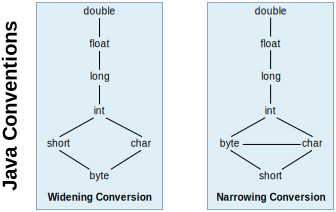
\includegraphics[width=.6\linewidth]{java_type_conversion}
	\end{center}
\end{frame}

\begin{frame}{{Implicit and Explicit} Type Conversions}
	\begin{definitionblock}{Implicit Conversion, or Coercion}
		Automatically done by the compiler, with a possible warning message in the case of narrowing conversion
	\end{definitionblock}
	\begin{itemize}
		\item Many languages limit the implicit conversions to \emph{widening conversions}
	\end{itemize}
	\vspace{1cm}
	\begin{definitionblock}{Explicit Conversion, or Cast}
		Conversions written in the source code by the programmer
	\end{definitionblock}
\end{frame}

\begin{frame}[t]{Function \ccode{maxType(t$_1$, t$_2$)}}
	\begin{definition}
		$\begin{array}{r@{}l}
			maxType : \mathbb{T} \times \mathbb{T} \rightarrow & \mathbb{T} \\
			(t_1, t_2) \mapsto & \text{maximum or least upper bounds of }t_1\text{ and }t_2 \\
			& \text{in the widening hierarchy; Otherwise error} \\
		\end{array}$
	\end{definition}
	\begin{example}
		\ccode{maxType(\kw{short}, \kw{char})} $\rightarrow$ \kw{int}
		\hspace{2em}
		\raisebox{-.9\height}{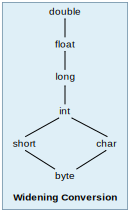
\includegraphics[width=.2\linewidth]{widening_type_conversion}}
	\end{example}
\end{frame}

\begin{frame}{Function \ccode{widenVar(a, t$_{out}$, t$_{in}$)}}
	\begin{definition}
		$\begin{array}{rl}
			widenVar : \mathbb{A} \times \mathbb{T} \times \mathbb{T} \rightarrow & \mathbb{A} \\
			(a, t_{out}, t_{in}) \mapsto & \text{Generates the code that widens the} \\
			& \text{value pointed by }a\text{ to the type }t_{out} \\[.2cm]
			& \text{Assuming that }a\text{ is of type }t_{in} \\[.2cm]
			& \text{Conversion is done only if it is required} \\[.2cm]
			& \text{Returns the address were the result} \\
			& \text{of the is available.} \\
		\end{array}$
	\end{definition}
\end{frame}

\begin{frame}{Example of Function \ccode{widenVar(a, t$_{out}$, t$_{in}$)}}
	Assume a language with only the two types \kw{int} and \kw{float}. \\
	\vspace{1em}
	\begin{myfunction}{widenVar}{a : $\mathbb{A}$, t$_{out}$ : $\mathbb{T}$, t$_{in}$ : $\mathbb{T}$}{$\mathbb{A}$}
		\Begin{
			\uIf{t$_{out}$ = t$_{in}$}{
				\Return a;
			}
			\uElseIf{t$_{in}$ = \kw{int} and t$_{out}$ = \kw{float}}{
				t \affect \kw{new} TemporaryVariable()\;
				\kw{quadruple}("(float)", a, $\emptyset$, t)\;
				\Return t
			}
			\Else{
				\throw{"Cannot widen the variable"}
			}
		}
	\end{myfunction}
\end{frame}

\begin{frame}{Function \ccode{narrowVar(a, t$_{out}$, t$_{in}$)}}
	\begin{definition}
		$\begin{array}{rl}
			narrowVar : \mathbb{A} \times \mathbb{T} \times \mathbb{T} \rightarrow & \mathbb{A} \\
			(a, t_{out}, t_{in}) \mapsto & \text{Generates the code that narrows the} \\
			& \text{value pointed by }a\text{ to the type }t_{out} \\[.2cm]
			& \text{Assuming that }a\text{ is of type }t_{in} \\[.2cm]
			& \text{Conversion is done only if it is required} \\[.2cm]
			& \text{Returns the address were the result} \\
			& \text{of the is available} \\
		\end{array}$
	\end{definition}
\end{frame}

\begin{frame}{Example of Function \ccode{narrowVar(a, t$_{out}$, t$_{in}$)}}
	Assume a language with only the two types \kw{int} and \kw{float}. \\
	\vspace{1em}
	\begin{myfunction}{narrowVar}{a : $\mathbb{A}$, t$_{out}$ : $\mathbb{T}$, t$_{in}$ : $\mathbb{T}$}{$\mathbb{A}$}
		\Begin{
			\uIf{t$_{out}$ $\neq$ \kw{int} or t$_{in}$ $\neq$ \kw{float}}{
				\throw{"Cannot narrow the variable"}
			}
			\uElseIf{t$_{out}$ = \kw{int} and t$_{in}$ = \kw{float}}{
				t \affect \kw{new} TemporaryVariable()\;
				\kw{quadruple}("(float)", a, $\emptyset$, t)\;
				\Return t
			}
			\Else{
				\Return a
			}
		}
	\end{myfunction}
\end{frame}

\begin{frame}{Example of Type Conversions in SDD}
	Attribute "\ccode{type}" is added to store the type of an expression \\
	SDD is updated to check the types: \\
	\vspace{1em}
	\begin{sdd}
		\sddprod{E}{\sddpn{E} \; \sddts{+} \; \sddpn{E}}{
			head.type = \alert{maxType}(E$_1$.type, E$_2$.type) \newl
			o1 = \alert{widenVar}(E$_1$.addr, E$_1$.type, head.type) \newl
			o2 = \alert{widenVar}(E$_2$.addr, E$_2$.type, head.type) \newl
			head.addr = \kw{new} TemporaryVariable() \newl
			\kw{quadruple}("+", o1, o2, head.addr)
		}
		\sddprod{E}{\sddts{id} \; \sddts{=} \; \sddpn{E}}{
			head.addr = SymbolTable.current.get(\sddts{id}.lexeme) \newl
			head.type = v.type \newl
			w = \alert{narrowVar}(E.addr, E.type, head.type) \newl
			\kw{if} (w $\neq$ E.addr) \newl
			\hspace{2em}\kw{warning}~"May loose information" \newl
			\kw{else} \newl
			\hspace{2em}w = \alert{widenVar}(E.addr, E.type, head.type) \newl
			\kw{quadruple}("=", w, $\emptyset$, head.addr)
		}
	\end{sdd}
\end{frame}

\subsubsection{Overloaded and polymorphic functions}
\subsubsectiontableofcontentslide

\begin{frame}{Overloading of a Function}
	\begin{definition}
		Allow the creation of several functions with the same name, which differ from each other in the type of the input and the output of the function
	\end{definition}
	\begin{itemize}
	\item Depending on the context, the overloading may be for a function, a procedure, a method, or an operator
	\vspace{.5cm}
	\item \Emph{Symbol table must contains all the signatures of the functions (in the context, which is using the symbol table)}
	\vspace{.5cm}
	\item A signature consists of:
		\begin{enumerate}
		\item the function name
		\item the list of the types of the formal parameters of the function
		\end{enumerate}
	\end{itemize}
\end{frame}

\begin{frame}{Polymorphic Function}
	\begin{definition}
			The term ``polymorphic'' refers to any code fragment that can be executed with arguments of different types
	\end{definition}
	\vspace{1cm}
	\alertbox{
		Only \emph{parametric polymorphism} is considered in this section \\
		where the polymorphism is characterized by parameters or type variables}
\end{frame}

\begin{frame}[background=8,fragile]{Example of Polymorphic Function}
	\begin{itemize}
	\item Consider the following definition in ML language:
		\begin{lstlisting}[language=ml]
fun length(x) = if null(x) then 0 else length( tl(x) ) + 1;
		\end{lstlisting}
	\vfill
	\item Consider the following statement in ML language:
		\begin{lstlisting}[language=ml]
length( ["sun", "mon", "tue"] ) + length( [10, 9, 8, 7] )
		\end{lstlisting}
	\vfill
	\item The same function \code{length()} is invoked on an array of strings and on an array of integers.
	\vfill
	\item The result of the ML statement is: \code{3 + 4 = 7}
	\end{itemize}
\end{frame}

\begin{frame}[background=9]{Type of a Polymorphic Function}
	\begin{itemize}
	\item Using the symbol $\forall$ and the type constructor \kw{list}, the type/signature of the function \ccode{length} is:
		\begin{center}
			$\forall a.\kw{list}(a) \rightarrow \kw{int}$
		\end{center}
	\vspace{.5cm}
	\item $\forall$ symbol is the universal quantifier, and the type variable to which it is applied is said to be bound by it
	\item Type expression with a $\forall$ symbol is referred as a ``polymorphic type''
	\vspace{.5cm}
	\item Each time a polymorphic function is applied, its bound type variables (a\dots) can denote a different type
	\end{itemize}
\end{frame}

\begin{frame}{{Determining the Type} of a Polymorphic Function}
	\alertbox{How to determine the types in the signature of a polymorphic function?}
	\vspace{1em}
	\alertbox*{
		We must infer the types by exploring the syntax tree of the function \newline
		and applying the substitution and unification operations}
	\begin{center}
		\titlebox*[.4\linewidth]{Substitution}{
			Mapping from type variables to type expressions \newline \emph{Example:} \kw{list}(\kw{int}) is an instance of \kw{list}($\alpha$), since it is the result of substituting \kw{int} for $\alpha$ in \kw{list}($\alpha$)
		}
		\hspace{1cm}
		\titlebox*[.4\linewidth]{Unification}{
			Determine whether type variables $s$ and $t$ are structurally equivalent by substituting the type variables in $s$ and $t$ by type expressions
		}
	\end{center}
\end{frame}

\begin{frame}[t,fragile]{Example of Type Inference on Polymorphic Function}
	\begin{columns}
		\begin{column}{.4\linewidth}
			\begin{small}
			\begin{lstlisting}[language=ml]
fun length(x) =
  if null(x) then 0
  else length( tl(x) ) + 1;
			\end{lstlisting}
			\end{small}
		\end{column}
		\begin{column}{.6\linewidth}
			\begin{scriptsize}
			\begin{tabularx}{\linewidth}{|X|X|X|}
				\hline
				\tabularheading\chead{Expression}&\chead{Type}&\chead{Unification} \\
				\hline
				\only<2->{length} & \only<2->{$\beta \rightarrow \gamma$} & \\
				\hline
				\only<2->{x} & \only<2->{$\beta$} & \\
				\hline
				\only<3->{\kw{if}} & \only<3->{$\mathbb{B} \times \alpha \times \alpha \rightarrow \alpha$} & \only<3->{$\alpha = \gamma$} \\
				\hline
				\only<4->{null} & \only<4->{$\kw{list}(\omega_n)\rightarrow\mathbb{B}$} & \\
				\hline
				\only<5->{null(x)} & \only<5->{$\mathbb{B}$} & \only<5->{$\kw{list}(\omega_n) = \beta$} \\
				\hline
				\only<6->{0} & \only<6->{\kw{int}} & \only<6->{$\alpha = \kw{int}$} \\
				\hline
				\only<7->{\kw{+}} & \only<7->{$\phi\times\phi\rightarrow\phi$} & \only<7->{$\phi = \alpha$} \\
				\hline
			\end{tabularx}
			\end{scriptsize}
		\end{column}
	\end{columns}
	\putat(100,-135){\includeanimatedfigure[width=.4\paperwidth]{unification_example}}
	\only<8>{\putat(-10,-120){\parbox{20em}{\mdseries\normalcolor\normalsize
		The type of the function "\code{length}" is: \\
		\code{length} : \kw{list}($\omega_n$) $\rightarrow$ \kw{int}
	}}}
\end{frame}

\section[Generation of statements]{Code generation of statements}
\sectiontableofcontentslide

\subsection{Control flow}
\subsectiontableofcontentslide

\begin{frame}{Control Flow}
	\alertbox{Translation of statements (if-else-statements, while-statements\dots) needs translation of boolean expressions}
	\vspace{.25cm}
	\begin{block}{Boolean expressions are used for:}
		\begin{center}
			\simplebox*[.4\linewidth]{\Emph{Altering the flow of control}}
			\hspace{1cm}
			\simplebox*[.4\linewidth]{Computing logical values}
		\end{center}
	\end{block}
	\begin{itemize}
	\item To support this distinction, we may:
		\begin{enumerate}
		\item Use two different nonterminals
		\item Use inherited attributes
		\item Use a set of flags during the parsing
		\item Build a syntax tree and invoke different procedures for the two different uses
		\end{enumerate}
	\end{itemize}
\end{frame}

\begin{frame}[t,fragile]{Short-Circuit Code}
	\begin{definition}
		Boolean operators are translated into \emph{jumps} \\
		These operators themselves do not appear in the three-address code
	\end{definition}
	\vspace{.25cm}
	\hiconbox{\smaller Value of a boolean expression is represented by a position in the code sequence}{note-icon}
	\vspace{.25cm}
	\begin{example}
		\begin{lstlisting}[style=lststyle-java]
if ( x < 100 || x > 200 && x != y ) x = 0;
		\end{lstlisting}
		\vspace{-.5cm}
		\begin{tac}[.6\linewidth]
		\ifgoto{$x < 100$}{L1}
		\ifnotgoto{$x > 200$}{L2}
		\ifnotgoto{$x \neq y$}{L2}
		\a[L1]{$x$}{$0$}
		\tacdots[L2]
		\end{tac}
	\end{example}
\end{frame}

\subsubsection{Translate the control flow statements}
\subsubsectiontableofcontentslide

\begin{frame}[background=6]{Statements for Control Flow}
	\begin{itemize}
	\item Consider the grammar: \\
		\begin{footnotesize}\begin{minipage}{.5\linewidth}
		\begin{bnf}
		\bnfprod*{S}{\bnfts{if} \; \bnfts{(} \; \bnfpn{B} \; \bnfts{)} \; \bnfpn{S}} \\
		\bnfalt*{\bnfts{if} \; \bnfts{(} \; \bnfpn{B} \; \bnfts{)} \; \bnfpn{S} \; \bnfts{else} \; \bnfpn{S}} \\
		\bnfalt*{\bnfts{while} \; \bnfts{(} \; \bnfpn{B} \; \bnfts{)} \; \bnfpn{S}}
		\end{bnf}
		\end{minipage}\end{footnotesize}
	\vspace{1cm}
	\item We introduce the attributes:
		\begin{itemize}
		\item \tactext{B.code} and \tactext{S.code}: synthesized attributes; three-address code of the nonterminals
		\item \tactext{B.true}: inherited attribute; the label of the code associated to the then-statements
		\item \tactext{B.false}: inherited attribute; the label of the code associated to the else-statements
		\item \tactext{B.next}: inherited attribute; the label of the code just after the current if-then-else statements
		\end{itemize}
	\end{itemize}
\end{frame}

\begin{frame}{Statement \kw{if}-\kw{then}}
	\begin{columns}
		\begin{column}{.4\linewidth}
			\pgfuseimage{statement-if}
		\end{column}
		\begin{column}{.6\linewidth}
			\begin{footnotesize}
			\begin{sdd}
			\sddprod{S}{\sddts{if} \; \sddts{(}}{
				B.true = \kw{newlabel}() \newl
				B.false = head.next
			}
			\sddmore{\sddpn{B} \; \sddts{)}}{
				S.next = head.next \newl
				\kw{label}(B.true)}
			\sddmore{\sddpn{S}}{}
			\end{sdd}
			\end{footnotesize}
		\end{column}
	\end{columns}
	\begin{itemize}
	\vfill
	\item Nonterminal for the condition is no more $E$ (nonterminal for expressions), but $B$ (specific nonterminal for boolean expressions in control flow)
	\item \tactext{newlabel()} creates a new label each time it is called
	\item \tactext{label($\alpha$)} attaches label $\alpha$ to the next three-address instruction to be generated
	\end{itemize}
\end{frame}

\begin{frame}{Statement \kw{if}-\kw{then}-\kw{else}}
	\begin{columns}
		\begin{column}{.4\linewidth}
			\pgfuseimage{statement-if-else}
		\end{column}
		\begin{column}{.6\linewidth}
			\begin{footnotesize}
			\begin{sdd}
			\sddprod{S}{\sddts{if} \; \sddts{(}}{
				B.true = \kw{newlabel}() \newl
				B.false = \kw{newlabel}()
			}
			\sddmore{\sddpn{B} \; \sddts{)}}{
				S$_1$.next = head.next \newl
				\kw{label}(B.true)
			}
			\sddmore{\sddpn{S} \; \sddts{else}}{
				\kw{quadruple}("goto", head.next, $\emptyset$, $\emptyset$) \newl
				S$_2$.next = head.next \newl
				\kw{label}(B.false)
			}
			\sddmore{\bnfpn{S}}{}
			\end{sdd}
			\end{footnotesize}
		\end{column}
	\end{columns}
\end{frame}

\begin{frame}{Statement \kw{while}}
	\begin{columns}
		\begin{column}{.4\linewidth}
			\pgfuseimage{statement-while}
		\end{column}
		\begin{column}{.6\linewidth}
			\begin{footnotesize}
			\begin{sdd}
			\sddprod{S}{\sddts{while} \; \sddts{(}}{
				begin = \kw{newlabel}() \newl
				B.true = \kw{newlabel}() \newl
				B.false = head.next
			}
			\sddmore{\sddpn{B} \; \sddts{)}}{
				S.next = begin \newl
				\kw{label}(B.true)
			}
			\sddmore{\sddpn{S}}{
				\kw{quadruple}("goto", begin, $\emptyset$, $\emptyset$)
			}
			\end{sdd}
			\end{footnotesize}
		\end{column}
	\end{columns}
\end{frame}

\subsubsection{Translate boolean expressions for control flow}
\subsubsectiontableofcontentslide

\begin{frame}{Boolean Constants in the Control Flow}
	\alertbox*{
		Boolean expressions for control flow need dedicated semantic rules
	}
	\vspace{.5cm}
	\hiconbox{Boolean expressions used in control-flow statements must be translated into jumping three-address code}{note-icon}
	\vspace{.5cm}
	\begin{sdd}
	\sddprod{B}{\sddts{true}}{
		\kw{quadruple}("goto", head.true, $\emptyset$, $\emptyset$)
	}
	\sddprod{B}{\sddts{false}}{
		\kw{quadruple}("goto", head.false, $\emptyset$, $\emptyset$)
	}
	\end{sdd}
\end{frame}

\begin{frame}{{Boolean Operator} NOT}
	\begin{columns}
		\begin{column}{.4\linewidth}
			\begin{center}
			\pgfuseimage{statement-not}
			\end{center}
		\end{column}
		\begin{column}{.6\linewidth}
			\begin{footnotesize}
			\begin{sdd}
			\sddprod{B}{\sddts{\string!} \; \sddpn{B}}{
				B.true = head.false \newl
				B.false = head.true
			}
			\end{sdd}
			\end{footnotesize}
		\end{column}
	\end{columns}
	\vfill
	\begin{itemize}
	\item No code is needed for an expression of the form \tactext{\tacts{\string!}B}
	\item Just interchange the \tactext{true} and \tactext{false} attributes of the head to set the \tactext{true} and \tactext{false} attributes of $B$
	\end{itemize}
\end{frame}

\begin{frame}{{Boolean Operator} OR}
	\begin{columns}
		\begin{column}{.45\linewidth}
			\pgfuseimage{statement-or}
		\end{column}
		\begin{column}{.55\linewidth}
			\begin{footnotesize}
			\begin{sdd}
			\sddprod{B}{}{
				B$_1$.true = head.true \newl
				B$_1$.false = \kw{newlabel}()
			}
			\sddmore{\sddpn{B}}{
				B$_2$.true = head.true \newl
				B$_2$.false = head.false
			}
			\sddmore{\sddts{\textbar\textbar} \; \sddpn{B}}{}
			\end{sdd}
			\end{footnotesize}
		\end{column}
	\end{columns}
	\vspace{.5cm}
	\begin{itemize}
	\item If $B_1$ is true, the head is true
	\item If $B_1$ is false, evaluate $B_2$
	\item So \tactext{B$_1$.false} is the label of the first instruction of \tactext{B$_2$}
	\item The value of the head becomes the same as the value of $B_2$
	\end{itemize}
\end{frame}

\begin{frame}{{Boolean Operator} AND}
	\begin{columns}
		\begin{column}{.45\linewidth}
			\pgfuseimage{statement-and}
		\end{column}
		\begin{column}{.55\linewidth}
			\begin{footnotesize}
			\begin{sdd}
			\sddprod{B}{}{
				B$_1$.true = \kw{newlabel}() \newl
				B$_1$.false = head.false
			}
			\sddmore{\sddpn{B}}{
				B$_2$.true = head.true \newl
				B$_2$.false = head.false
			}
			\sddmore{\sddts{\&\&} \; \sddpn{B}}{}
			\end{sdd}
			\end{footnotesize}
		\end{column}
	\end{columns}
	\vfill
	\begin{itemize}
	\item If $B_1$ is false, the head is false
	\item If $B_1$ is true, evaluate $B_2$
	\item So \tactext{B$_1$.true} is the label of the first instruction of $B_2$
	\item The value of the head becomes the same as the value of $B_2$
	\end{itemize}
\end{frame}

\begin{frame}{Comparison Operators}
	\begin{columns}
		\begin{column}{.3\linewidth}
			\begin{center}
			\pgfuseimage{statement-comparison}
			\end{center}
		\end{column}
		\begin{column}{.7\linewidth}
			\begin{footnotesize}
			\begin{sdd}
			\sddprod{B}{\sddpn{E} \; \sddts{rel} \; \sddpn{E}}{
				t = \kw{new} TemporaryVariable() \newl
				\kw{quadruple}(\sddts{rel}.operator, \newl
				\hspace{1em}E$_1$.addr, E$_2$.addr, t) \newl
				\kw{quadruple}("if", t, \newl
				\hspace{1em}head.true, $\emptyset$) \newl
				\kw{quadruple}("goto", head.false, \newl
				\hspace{1em}$\emptyset$, $\emptyset$)}
			\end{sdd}
			\end{footnotesize}
		\end{column}
	\end{columns}
	\vspace{.5cm}
	\begin{itemize}
	\item Form $a<b$ is translated to: \\
		\tactext{t = ($a<b$)} \\
		\tactext{\kw{if} t \kw{then} \kw{goto} B.true} \\
		\tactext{\kw{goto} B.false} \\
	\end{itemize}
\end{frame}

\begin{frame}[fragile]{Example of Translation}
	\begin{lstlisting}[style=lststyle-java]
		if ( x < 100 || x > 200 && x != y ) x = 0;
	\end{lstlisting}
	\vfill
	\begin{tac}
	\a{\t1}{$x < 100$}
	\ifgoto{\t1}{L2}
	\goto{L3}
	\a[L3]{\t1}{$x > 200$}
	\ifgoto{$x > 200$}{L4}
	\goto{L1}
	\a[L4]{\t1}{$x \neq y$}
	\ifgoto{\t1}{L2}
	\goto{L1}
	\a[L2]{x}{0}
	\tacdots[L1]
	\end{tac}
\end{frame}

\subsubsection{Avoid redundant goto}
\subsubsectiontableofcontentslide

\begin{frame}[background=8]{Redundant Goto Statements}
	\begin{small}
	\alertbox{The semantic rules described in the previous slides \newline
		may generate more goto instructions than strictly necessary}
	\vspace{.5cm}
	\begin{example}
		\begin{tac}
		\a[L3]{\t1}{$x>200$}
		\ifgoto{\t1}{L4}
		\goto{L1}
		\tacdots[L4]
		\tacdots[L1]
		\end{tac}
	\end{example}
	\vspace{.5cm}
	\begin{block}{Best Practice}
		\begin{tac}
		\a[L3]{\t1}{$x>200$}
		\ifnotgoto{\t1}{L1}
		\tacdots
		\tacdots[L1]
		\end{tac}
	\end{block}
	\end{small}
\end{frame}

\begin{frame}{Remove Redundant Gotos}
	\hiconbox{
		Avoiding redundant gotos is done by introducing a constant for the value of the labels: \tactext{fall} \newline
		It means ``don't generate any jump'' or ``fall in the next available instruction''
	}{method-icon}
	\vspace{.25cm}
	\alertbox{We can adapt the semantic rules of the boolean expressions. $\bnfpn{S} \bnfopo \bnfts{if} \; \bnfts{(} \; \bnfpn{B} \; \bnfts{)} \; \bnfpn{S}$}
	\vspace{.25cm}
	\begin{tabularx}{\linewidth}{@{}XcX@{}}
		\begin{small}
		\begin{sdd}
		\sddprod{S}{\sddts{if} \; \sddts{(}}{
			B.true = \kw{newlabel}() \newl
			B.false = head.next
		}
		\sddmore{\sddpn{B} \; \sddts{)}}{
			S.next = head.next \newl
			\kw{label}(B.true)
		}
		\sddmore{\sddpn{S}}{}
		\end{sdd}
		\end{small}
		& \pgfuseimage{right-arrow}
		&
		\begin{small}
		\begin{sdd}
		\sddprod{S}{\sddts{if} \; \sddts{(}}{
			B.true = \kw{fall} \newl
			B.false = head.next
		}
		\sddmore{\sddpn{B} \; \sddts{)}}{
			S.next = head.next
		}
		\sddmore{\sddpn{S}}{}
		\end{sdd}
		\end{small}
	\end{tabularx}
\end{frame}

\begin{frame}[t]{Remove Redundant Gotos of the OR Operator}
	\begin{center}
		\begin{sdd}[.8\linewidth]
		\sddprod{B}{}{
			B$_1$.true = head.true \newl
			B$_1$.false = \kw{newlabel}()
		}
		\sddmore{B}{
			B$_2$.true = head.true \newl
			B$_2$.false = head.false
		}
		\sddmore{\sddts{\textbar\textbar} \; \sddpn{B}}{}
		\end{sdd} \\[.1cm]
		\pgfuseimage{bottom-arrow} \\[.1cm]
		\begin{sdd}[.8\linewidth]
		\sddprod{B}{}{
			\kw{if} head.true = \kw{fall} \newl
			\hspace{1em}B$_1$.true = newlabel() \newl
			\kw{else} \newl
			\hspace{1em}B$_1$.true = head.true \newl
			B$_1$.false = \kw{fall}
		}
		\sddmore{\sddpn{B}}{
			B$_2$.true = head.true \newl
			B$_2$.false = head.false
		}
		\sddmore{\sddts{\textbar\textbar} \; \sddpn{B}}{
			\kw{if} head.true = \kw{fall} \newl
			\hspace{1em}label(B$_1$.true)
		}
		\end{sdd}
	\end{center}
\end{frame}

\subsection{Backpatching}

\subsubsection{Introduction}
\subsubsectiontableofcontentslide

\begin{frame}{Problem with Jumps}
	\alertbox{
		A key problem is the matching of a jump instruction \newline
		with the target address of the jump
	}
	\vspace{1em}
	\begin{example}
		\begin{itemize}
		\item Consider the statement $\bnfts{if} \; \bnfts{(} \; \bnfpn{B} \; \bnfts{)} \; \bnfpn{S}$
		\item In a \emph{one-pass translation}, $B$ must be translated before $S$ is examined
		\item \alert{What is the address of the label that permits to go over the code for $S$?}
		\end{itemize}
	\end{example}
\end{frame}

\begin{frame}{Solving the Problem with Jumps}
	\begin{block}{Solution 1}
		\begin{itemize}
			\item In the previous slides, we solve this problem by using inherited attribute "\texttt{next}"
			\item \alert{But a separate (additionnal) pass is then needed to bind labels to addresses}
		\end{itemize}
	\end{block}
	\vspace{1cm}
	\begin{block}{Solution 2}
		\begin{itemize}
			\item \emph{Backpatching} can be used to generate code for boolean expressions and flow-of-control statements in one pass
			\item This approach is detailled in the following slides
		\end{itemize}
	\end{block}
\end{frame}

\begin{frame}{General Principle of Backpatching}
	\begin{rightarrowsequence}
		\arrow[bg=CIADlightgray,fg=black]{
			When the jump target is after the current instruction \\[.5cm]
			Address of the current instruction is added into a list
		}
		\arrow[bg=CIADdarkgray]{
			When the address of the target instruction is known \\[.5cm]
			Instructions in the list are updated
		}
	\end{rightarrowsequence}
	\vspace{.5cm}
	New synthesized attributes in $B$:
	\begin{description}
		\item[B.bptruelist] list of jump or conditional jump instructions into which we must insert the label to which control goes if $B$ is true.
		\vfill
		\item[B.bpfalselist] list of instructions that eventually get the label to which control goes when $B$ is false.
	\end{description}
\end{frame}

\begin{frame}[background=9]{Tools for the Backpatching}
	\begin{description}
	\item[makebplist(adr)] creates a new list containing only $adr$, an index into the array of instructions
	\vfill
	\item[mergebplists(lst1,lst2)] concatenates the lists pointed by $lst1$ and $lst2$, and returns a pointer to the result
	\vfill
	\item[backpatch(lst,adr)] inserts $adr$ as the target label for each of the instructions on the list pointed to by $lst$
	\vfill
	\item[instadr()] replies the address of the instruction that will be generated by the \Emph{next} call to \tactext{\kw{quadruple}()}
	\vfill
	\item[Unknown address] Keyword \kw{?} represents an unkwown address
	\end{description}
\end{frame}

\begin{frame}{Backpatching of the Boolean Control-Flow Rules}
	\begin{sdd}
	\sddprod{B}{\sddpn{true}}{
		\emph{head.bptruelist = makebplist(instadr())} \newl
		\kw{quadruple}("goto", \emph{\kw{?}}, $\emptyset$, $\emptyset$)
	}
	\hline
	\sddprod{B}{\sddts{false}}{
		\emph{head.bpfalselist = makebplist(instadr())} \newl
		\kw{quadruple}("goto", \emph{\kw{?}}, $\emptyset$, $\emptyset$)
	}
	\hline
	\sddprod{B}{\sddpn{E} \; \sddts{rel} \; \sddpn{E}}{
		t = \kw{new} TemporaryVariable() \newl
		\kw{quadruple}(\sddts{rel}.operator, E$_1$.addr, E$_2$.addr, t) \newl
		\emph{head.bptruelist = makebplist(instadr())} \newl
		\kw{quadruple}("if", t, \emph{\kw{?}}, $\emptyset$) \newl
		\emph{head.bpfalselist = makebplist(instadr())} \newl
		\kw{quadruple}("goto", \emph{\kw{?}}, $\emptyset$, $\emptyset$)
	}
	\hline
	\sddprod{B}{\sddpn{B} \; \sddts{\textbar\textbar}}{
		\emph{\kw{backpatch}(B$_1$.bpfalselist, instadr())}
	}
	\sddmore{\sddpn{B}}{
		\emph{head.bptruelist = mergbplists(} \newl
		\hspace{1em}\emph{B$_1$.bptruelist, B$_2$.bptruelist)} \newl
		\emph{head.bpfalselist = B$_2$.bpfalselist}
	}
	\end{sdd}
\end{frame}

\begin{frame}{Backpatching of the Control-Flow Statements}
	\begin{sdd}
	\sddprod{S}{\sddts{if} \; \sddts{(} \; \sddpn{B} \; \sddts{)}}{
		backpatch(B.bptruelist, instadr())
	}
	\sddmore{\sddpn{S}}{
		head.\emph{bpnextlist} = mergebplists(B.bpfalselist, S.\emph{bpnextlist})
	}
	\hline
	\sddprod{S}{\sddts{if} \; \sddts{(} \; \sddpn{B} \; \sddts{)}}{
		backpatch(B.bptruelist, instadr())
	}
	\sddmore{\sddpn{S} \; \sddts{else}}{
		backpatch(B.bpfalselist, instadr())
	}
	\sddmore{\sddpn{S}}{
		head.\emph{bpnextlist} = mergebplists(S$_1$.\emph{bpnextlist}, S$_2$.\emph{bpnextlist})
	}
	\hline
	\sddprod{S}{\sddts{while}}{
		a = instadr()
	}
	\sddmore{\sddts{(} \; \sddpn{B} \; \sddts{)}}{
		backpatch(B.bptruelist, instadr())
	}
	\sddmore{\sddpn{S}}{
		backpatch(S.\emph{bpnextlist}, a) \newl
		\kw{quadruple}("goto", a, $\emptyset$, $\emptyset$) \newl
		head.\emph{bpnextlist} = B.bpfalselist
	}
	\end{sdd}
	\vspace{.5cm}
	The attribute \tactext{bpnextlist} is the list of the addresses of the instructions that are refering the ``next instruction''
\end{frame}

\begin{frame}[t]{Algorithm of \ccode{backpatch()}}
	\begin{footnotesize}
	\begin{myprocedure}{backpatch}{list, address}
	\Input{$\mathbb{Q}$ is the global list of the generated quadruples}
	\Begin{
		\ForEach{$a \in list$}{
			q \affect $\mathbb{Q}[a]$\;
			\uIf{q.op = "goto"}{
				\lIf{q.arg$_1$ $\neq$ \kw{?}}{\throw{"Cannot backpatch"}}
				q.arg$_1$ \affect address\;
			}
			\uElseIf{q.op = "if"}{
				\lIf{q.arg$_2$ $\neq$ \kw{?}}{\throw{"Cannot backpatch"}}
				q.arg$_2$ \affect address\;
			}
			\uElseIf{q.op = "ifFalse"}{
				\lIf{q.arg$_2$ $\neq$ \kw{?}}{\throw{"Cannot backpatch"}}
				q.arg$_2$ \affect address\;
			}
			\Else{
				\throw{"Instruction to backpatch not found"}
			}
		}
	}
	\end{myprocedure}
	\end{footnotesize}
\end{frame}

\section{Conclusion}
\sectiontableofcontentslide

\begin{frame}{{Key Concepts} in the Chapter}
	\begin{description}
	\item[Inherited and synthesized attributes] Syntax-directed definitions may use two kinds of attributes. A synthesized attribute at a parse-tree node is computed from attributes at its children. An inherited attribute at a node is computed from attributes at its parent and/or siblings
	\item[Dependency graphs] Given a parse tree and an SDD, we draw edges among the attribute instances associated with each parse-tree node to denote that the value of the attribute at the head of the edge is computed in terms of the value of the attribute at the tail of the edge
	\item[S-Attributed definitions] In a S-attributed SDD, all attributes are synthesized
	\item[L-Attributed definitions] In a L-attributed SDD, attributes may be inherited or synthesized. However, inherited attributes at a parse-tree node may depend only on inherited attributes of its parent and on (any) attributes of siblings to its left
	\item[Syntax trees] Each node in a syntax tree represents a construct; the children of the node represent the meaningful components of the construct
	\end{description}
\end{frame}

\begin{frame}{{Key Concepts} in the Chapter \insertcontinuationtext}
	\begin{description}
	\item[Intermediate representation] An intermediate representation is typically some combination of a graphical notation and three-address code. As in syntax, a node in a graphical notation represents a construct; the children of a node represent its subconstructs. Three address code takes its name from instructions of the form \tactext{x = y \kw{op} z}, with at most one operator per instruction. There are additional instructions for control flow
	\item[Translate expressions] Expressions with built-up operations can be unwound into a sequence of individual operations by attaching actions to each production of the form $E \bnfopo E_1 \bnfts{op} E_2$. The action either creates a node for $E$ with the nodes for $E_1$ and $E_2$ as children, or it generates a three-address instruction that applies op to the addresses for $E_1$ and $E_2$ and puts the result into a new temporary name, which becomes the address of $E$
	\end{description}
\end{frame}

\begin{frame}{{Key Concepts} in the Chapter \insertcontinuationtext}
\begin{description}
	\item[Check types] The type of an expression \tactext{E$_1$ \kw{op} E$_1$} is determined by the operator \kw{op} and the types of \tactext{E$_1$} and \tactext{E$_2$}. A coercion is an implicit type conversion. Intermediate code contains explicit type conversions to ensure an exact match between operand types and the types expected by an operator
	\item[Generate jumping code for boolean expression] In short-circuit or jumping code, the value of a boolean expression is implicit in the position reached in the code. Jumping code is useful because a boolean expression $B$ is typically used to \tactext{t=true} or \tactext{t=false}, as appropriate, where \tactext{t} is a temporary name. Using labels for jumps, a boolean expression can be translated by inheriting labels corresponding to its true and false exits attributes. The constants \kw{true} and \kw{false} translate into a jump to the true and false attributes, respectively
	\end{description}
\end{frame}

\begin{frame}{{Key Concepts} in the Chapter \insertcontinuationtext}
\begin{description}
	\item[Implement statements using control flow] Statements can be translated by inheriting a label next, where next marks the first instruction after the code for this statement. The conditional $\bnfpn{S} \bnfopo \bnfts{if} \bnfts{(} \bnfpn{B} \bnfts{)} \bnfpn{S}$ can be translated by attaching a new label marking the beginning of the code for $S$ and passing the new label and \tactext{S.next} for the true and false attributes, respectively, of $B$
	\item[Alternatively, use backpatching] Backpatching is a technique for generating code for boolean expressions and statements in one pass. The idea is to maintain lists of incomplete jumps, where all the jump instructions on a list have the same target. When the target becomes known, all the instructions on its list are completed by filling in the target
	\item[Implement records] Field names in a record or class can be treated as a sequence of declarations. A record type encodes the types and relative addresses of the fields. A symbol table object can be used for this purpose
	\end{description}
\end{frame}

\begin{frame}[t,fancyframetitle=false,allowframebreaks]{\bibname\ of the Chapter}%
	\tiny%
	\putbib[chapters/chapter4/biblio]%
\end{frame}%

\end{bibunit}
\end{graphicspathcontext}

\endinput
